%\documentclass[11pt,a4paper,oneside]{report}

\documentclass[12pt,a4paper,twoside,openright]{report}
\usepackage{amsmath}
\usepackage{graphicx} % Duplex
%\usepackage{hyperref}             % Single-side
% thanks to http://tex.stackexchange.com/a/47579/71109
\usepackage{ifxetex}
\usepackage{ifluatex}
\newif\ifxetexorluatex % a new conditional starts as false
\ifnum 0\ifxetex 1\fi\ifluatex 1\fi>0
   \xetexorluatextrue
\fi

\ifxetexorluatex
  \usepackage{fontspec}
\else
  \usepackage[T1]{fontenc}
  \usepackage[utf8]{inputenc}
  \usepackage[lighttt]{lmodern}
  \ttfamily\DeclareFontShape{T1}{lmtt}{m}{it}{<->sub*lmtt/m/sl}{}
\fi

\usepackage[english,magyar]{babel} % Alapértelmezés szerint utoljára definiált nyelv lesz aktív, de később külön beállítjuk az aktív nyelvet.

\usepackage{emptypage} % omit page number on empty pages

%\usepackage{cmap}
\usepackage{amsfonts,amsmath,amssymb} % Mathematical symbols.
%\usepackage[ruled,boxed,resetcount,linesnumbered]{algorithm2e} % For pseudocodes. % beware: this is not compatible with LuaLaTeX, see http://tex.stackexchange.com/questions/34814/lualatex-and-algorithm2e
\usepackage{booktabs} % For publication quality tables for LaTeX
\usepackage{graphicx}

%\usepackage{fancyhdr}
%\usepackage{lastpage}

\usepackage{geometry}
%\usepackage{sectsty}
\usepackage{setspace} % For setting line spacing

\usepackage[unicode]{hyperref} % For hyperlinks in the generated document.
\usepackage{xcolor}
\usepackage{listings} % For source code snippets.

\usepackage{pdfpages}
\usepackage[amsmath,thmmarks]{ntheorem} % Theorem-like environments.

\usepackage[hang]{caption}
\usepackage{subcaption}

\singlespacing

\newcommand{\selecthungarian}{
	\selectlanguage{magyar}
	\setlength{\parindent}{2em}
	\setlength{\parskip}{0em}
	\frenchspacing
}

\newcommand{\selectenglish}{
	\selectlanguage{english}
	\setlength{\parindent}{0em}
	\setlength{\parskip}{0.5em}
	\nonfrenchspacing
	\renewcommand{\figureautorefname}{Figure}
	\renewcommand{\tableautorefname}{Table}
	\renewcommand{\partautorefname}{Part}
	\renewcommand{\chapterautorefname}{Chapter}
	\renewcommand{\sectionautorefname}{Section}
	\renewcommand{\subsectionautorefname}{Section}
	\renewcommand{\subsubsectionautorefname}{Section}
}

\usepackage[numbers]{natbib}
\usepackage{xspace}


%TODO Set the main variables
\newcommand{\vikszerzoVezeteknev}{Nyilas}
\newcommand{\vikszerzoKeresztnev}{Péter}

\newcommand{\vikkonzulensAMegszolitas}{dr.~}
\newcommand{\vikkonzulensAVezeteknev}{Hullám}
\newcommand{\vikkonzulensAKeresztnev}{Gábor}

\newcommand{\vikcim}{
Training and Interpretation of a
Neural Network Model for
Traffic Object Detection
}

% Cím
\newcommand{\viktanszek}{\bmemit} % Tanszék
\newcommand{\vikdoktipus}{\bsc} % Dokumentum típusa (\bsc vagy \msc)
\newcommand{\vikmunkatipusat}{szakdolgozatot} % a "hallgató nyilatkozat" részhez: szakdolgozatot vagy diplomatervet

%\input{include/tdk-variables}
\newcommand{\szerzoMeta}{\vikszerzoVezeteknev{} \vikszerzoKeresztnev} % egy szerző esetén
%\newcommand{\szerzoMeta}{\vikszerzoVezeteknev{} \vikszerzoKeresztnev, \tdkszerzoB} % két szerző esetén

%TODO Language configuration -- choose one
% Beállítások magyar nyelvű dolgozathoz
%\input{include/thesis-hu}
% Settings for English documents
\input{include/thesis-en}

\input{include/preamble}

%--------------------------------------------------------------------------------------
% Table of contents and the main text
%--------------------------------------------------------------------------------------
\begin{document}
\begin{spacing}{1.2}

\pagenumbering{gobble}

%TODO These includes define guidelines -- remove these
%~~~~~~~~~~~~~~~~~~~~~~~~~~~~~~~~~~~~~~~~~~~~~~~~~~~~~~~~~~~~~~~~~~~~~~~~~~~~~~~~~~~~~~
%\include{include/guideline}
%\include{include/project}

\includepdf{include/Kozlekedesi-objektumok-detekciojat-megvalosito-Feladatkiiras.pdf}

\selectthesislanguage

%~~~~~~~~~~~~~~~~~~~~~~~~~~~~~~~~~~~~~~~~~~~~~~~~~~~~~~~~~~~~~~~~~~~~~~~~~~~~~~~~~~~~~~
\hypersetup{pageanchor=false}
%--------------------------------------------------------------------------------------
%	The title page
%--------------------------------------------------------------------------------------
\begin{titlepage}
\begin{center}
\includegraphics[width=60mm,keepaspectratio]{figures/bme_logo.pdf}\\
\vspace{0.3cm}
\textbf{\bme}\\
\textmd{\vik}\\
\textmd{\viktanszek}\\[5cm]

\vspace{0.4cm}
{\huge \bfseries \vikcim}\\[0.8cm]
\vspace{0.5cm}
\textsc{\Large \vikdoktipus}\\[4cm]

{
	\renewcommand{\arraystretch}{0.85}
	\begin{tabular}{cc}
	 \makebox[7cm]{\emph{\keszitette}} & \makebox[7cm]{\emph{\konzulens}} \\ \noalign{\smallskip}
	 \makebox[7cm]{\szerzo} & \makebox[7cm]{\vikkonzulensA} \\
	  %& \makebox[7cm]{\vikkonzulensB} \\
	  %& \makebox[7cm]{\vikkonzulensC} \\
	\end{tabular}
}

\vfill
{\large \today}
\end{center}
\end{titlepage}
\hypersetup{pageanchor=false}

		   % Szakdolgozat/Diplomaterv címlap

\renewcommand{\thesection}{\arabic{section}}
\renewcommand{\thesubsection}{\thesection.\arabic{subsection}}
\renewcommand{\thesubsubsection}{\thesubsection.\arabic{subsubsection}}
% Table of Contents
%~~~~~~~~~~~~~~~~~~~~~~~~~~~~~~~~~~~~~~~~~~~~~~~~~~~~~~~~~~~~~~~~~~~~~~~~~~~~~~~~~~~~~~
\tableofcontents\cleardoublepage


% Declaration and Abstract
%~~~~~~~~~~~~~~~~~~~~~~~~~~~~~~~~~~~~~~~~~~~~~~~~~~~~~~~~~~~~~~~~~~~~~~~~~~~~~~~~~~~~~~
\include{include/declaration} %TODO Hallgatói nyilatkozat
\pagenumbering{roman}
\setcounter{page}{1}

\selecthungarian

%----------------------------------------------------------------------------
% Abstract in Hungarian
%----------------------------------------------------------------------------
\chapter*{Kivonat}\addcontentsline{toc}{chapter}{Kivonat}

Ez a dokumentum egy mesterséges intelligencia alapú rendszer fejlesztését mutatja be, amely képes automatikusan
felismerni és osztályozni különböző objektumokat képeken, illetve foglalkozik a neurális hálózat interpretálásával.
A rendszer a YOLOv8 modelt használja, amely egy mély neurális hálózat alapú objektumfelismerő algoritmus.
A dolgozat részletesen tárgyalja a modell betanításának és interpretálásának folyamatát, valamint az elért eredményeket
és levonja a következtetéseket.

\vfill
\selectenglish

%----------------------------------------------------------------------------
% Abstract in English
%----------------------------------------------------------------------------
\chapter*{Abstract}\addcontentsline{toc}{chapter}{Abstract}

This paper describes the development of an artificial intelligence-based system that can
recognise and classify different objects in images and interprets the neural network.
The system uses the YOLOv8 model, which is a deep neural network based object recognition algorithm.
The paper discusses in detail the process of training and interpreting the model and the results obtained
and draws conclusions.

\vfill
\cleardoublepage

\selectthesislanguage

\newcounter{romanPage}
\setcounter{romanPage}{\value{page}}
\stepcounter{romanPage}    %TODO Összefoglaló


% The main part of the thesis
%~~~~~~~~~~~~~~~~~~~~~~~~~~~~~~~~~~~~~~~~~~~~~~~~~~~~~~~~~~~~~~~~~~~~~~~~~~~~~~~~~~~~~~
\pagenumbering{arabic}

%\subsection{Introduction and Motivations}\label{subsec:introduction-and-motivations} % bevezetés és motivációk
%értelmezés

\section{Introduction}\label{sec:introduction}

The accurate detection of objects that are relevant to vehicle control is a critical task in the field of automotive and transportation systems.
It is a particularly important aspect for the development of highly sophisticated autonomous driving systems, where numerous scenarios can arise in with different types of objects to detect and react to.
These objects can be either static (not moving), or dynamic (capable of moving).
The object detection is implemented trough the help of sensors using different physical phenomenons, such as acoustic or electromagnetic wave.
These sensors are mounted onto the chassis of the autonomous vehicle.

One of the most widely used solution is the use of camera sensors as they are able to
provide rich visual data that can be processed rapidly and can give the most information by itself.
The main goal of this project was to develop a software capable of detecting dynamic traffic
objects, while staying robust and reliable in various conditions.
A fitting solution for this task was to utilise deep learning models, especially Convolutional Neural Networks, CNNs for short.

%értelmezés
Nevertheless, the most significant limitation of these models is that they are frequently regarded as black boxes, lacking a straightforward correlation between input and output.
As we might want to use these systems in a safety critical applications,
it is important to avoid unpredictable behaviour or mistrust from the stakeholders.
High level of explainability should be the bases for trust and confidence between the system and its stakeholders.
In accordance with this, the artificial intelligence-functional safety and AI systems ISO standard\cite{ISO5469:2021} devotes a chapter(8.3) to
Degree of transparency and explainability.
These needs led to the development of numerous model interpretation techniques,
as evidenced by the work of a number of different researchers such as Yu Liang~\cite{LIANG2021168}.
These techniques vary in their approach, but they are all aiming to facilitate an insight into the decision-making process of the model.
In a unified manner, these methods are called eXplainable Artificial Intelligence methods, XAI for short.


%feladat indokoltsága
The complexity of interpreting models in these domains arises from two key factors: the intricate nature of the data and the sheer size of models used.
The aforementioned complexity makes it challenging to trace the decision-making process, which unfolds across numerous neurons and layers,
presents a significant challenge.
Nevertheless, it is essential for the identification of potential biases, the improvement of model performance, the fostering the trust of users and regulatory bodies.
These factors are particularly important in the context of traffic object detection, where the consequences of model errors can be severe.
This has heightened the importance of XAI solutions, with the aim of ensuring transparency for end users and developers alike.

As previously discussed in relation to other challenges facing the development of AI systems by Arun Das and Paul Rad in their article
\("\)Opportunities and Challenges in the Development of AI Systems\("\) ~\cite{das2020opportunitieschallengesexplainableartificial}
The General Data Protection Regulation (GDPR) now requires that decisions made by automated systems be
explainable to the user.
Although the GDPR does not explicitly mention XAI and mainly focuses on data privacy,
it seems probable that in the future, there will be a greater expectation of algorithmic transparency and clarification of AI systems.

%tervezés célja
It is therefore essential to enhance the interpretability of this project's model through the use of the aforementioned
XAI methods such as SHAP, LIME and EigenCAM in order to maintain safety and ethical standards, given the nature of the
application.
Based on that the secondary objective of this project was to try and implement these interpretation methods and examine their
effectiveness in the context of traffic object detection and try to instate a more transparent and reliable model.

\subsection{Refinement of the task}\label{subsec:Refinement-of-the-task} % feladat finomítása


The principal objective of this project is to develop a software solution capable of detecting traffic objects in real time.
This will entail an investigation into the fundamental principles of deep learning models for object detection, with a
particular emphasis on the construction of a model based on the YOLOv8 architectural framework.
The model will be trained on a dataset comprising images of urban environments, each of which has been annotated with
traffic objects.
Following training, the model's performance will be evaluated based on its capacity to accurately detect traffic objects
in real scenarios.

In addition to object detection, the secondary objective of the project is to enhance the interpretability of the
model through the utilisation of Explainable AI (XAI) me\-tho\-do\-lo\-gies.
The selection and implementation of both model-agnostic and model-specific interpretation techniques will be undertaken (they will be discussed and explained later),
with a particular focus on understanding their underlying principles and applying them to the traffic detection model.
The effectiveness of these interpretation techniques will be evaluated based on their
ability to provide insights into the rationale behind the model's predictions.
This will ensure that the system is both accurate and transparent in its decision-making processes.
The objective of this project is to develop a deep learning model for traffic object detection and to apply XAI methods to enhance the model's interpretability.

The two tasks were approached as discrete entities, and thus their explanations were presented separately.
Initially, the object detection and the neural network's fulfilment of the task and its evaluation were discussed.
Subsequently, the model's interpretation methods and their outcomes were evaluated.

The choice of dataset, model and interpretation methods was made with these goals in mind, with the intention of optimizing the model for the task in question, in line with the findings of the literature and previous studies.

\subsection{Structure}\label{subsec:Structure} % felépítés rövid összefoglalása

The main parts of my thesis are as follows:

\begin{itemize}
    \item Object detection component:
    \begin{itemize}
        \item Literature study about image processing Deep Convolutional Neural Networks.
        \item Yolo architecture and general overview on training and infrastructure.
        \item Cityscapes dataset and data processing and representation.
        \item Evaluation of model performance.
    \end{itemize}
    \item Interpretation methods
    \begin{itemize}
        \item Literature review about model-agnostic and model-dependent interpretation methods.
        \item Implementation, use and evaluation of EigenCAM, LIME and SHAP\@.
        \item To analyze the results and draw conclusions on the effectiveness of the model and the XAI solutions for traffic object detection.
    \end{itemize}
\end{itemize}
%TODO
%\section{Introduction to deep learning}\label{sec:introduction-to-deep-%learning} % bevezetés a mélytanulásba
%Új ötlet lehet nem árt egy overview a mélytanulásról, hogy aki nem ért hozzá az is tudja miről van szó

\newpage

\section{Image Processing Deep Neural Networks}\label{sec:image-processing-deep-neural-networks}

%Checked
\subsection{Overview of Convolutional Neural Networks}\label{subsec:convolutional-neural-networks}

CNNs constitute a class of deep learning models that are commonly used for computer vision tasks
including image classification, object detection, and semantic or instance segmentation.
Given the ability of convolutional neural networks to learn spatial hierarchies of features and their various types of data representations
(bounding box, segmentation mask, etc.), they are made ideal for the task of traffic object detection.
Many recent advances  in computer vision have been made possible by CNNs, including the development of models such as Yolo, Faster R-CNN, and SSD.
A dozen of these models have been developed, each with its own unique architecture and capabilities.
However, they all share the same fundamental principles gathered recently by Jiuxiang Gu in his 2018 work,
\("\)Recent advances in convolutional neural networks\("\)~\cite{GU2018354}.

The designation of the class is derived from the utilisation of convolutional layers,
which apply filters to the input data in order to extract features.
Additionally, convolutional neural networks comprise other layers, including
pooling layers, fully connected layers, and so forth.

These models are employed in a multitude of applications, including the perception
component in autonomous vehicles, surveillance systems, and medical imaging.
In view of the fact that these applications are in alignment with the project's stated objectives,
and given that the dataset in question is derived from a number of different urban traffic
environments, it has been decided that these types of neural networks should be employed for the
specific task of traffic object detection

The subsequent paragraphs will provide an overview of the essential components of convolutional neural networks.

\paragraph{Convolutional layers}\label{par:convolutional-layers}
represent the fundamental building blocks of convolutional neural networks.
Convolution operations are applied to the input data using filters (or in other word kernels) that process the input image.
This process enables the model to identify local patterns such as  edges, textures, and shapes.
Each convolutional layer generates a set of feature maps,
which indicate the presence of different types of these aforementioned features in the input.
These feature maps are then passed to the subsequent layers for further processing, such operations as pooling or classification,
to refine the information coded into the image.
During the training phase, the parameters of the kernels are learned (their values are adjusted), through backpropagation,
allowing the network to enhance feature extraction for specific tasks.


\begin{figure}[ht]
\centering
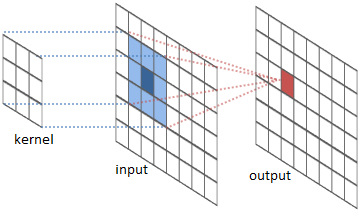
\includegraphics[width=.50\textwidth]{figures/convolution}
\caption{Convolutional layer operation~\cite{article}}
\label{fig:convolution}
\end{figure}

\paragraph{Fully connected layers}\label{par:fully-connected-layers}

is used to describe a type of neural network in which each
neuron is connected to every other neuron in the network's preceding layer, resulting in a dense connectivity pattern.
This connectivity pattern is also referred to as a "dense layer" due to its dense connections on the semantic figure.
They are typically located at the conclusion (HEAD) of convolutional neural network (CNN) architectures, where the final output is calculated.
In these layers, as one neuron receives data from every neuron in the previous layer, each connection characterised by a specific trainable weight and each neuron possesses a unique trainable bias.
This structure enables the model to integrate information from all features and make final predictions.
Fully connected layers in image processing or object detection tasks are computing the output probabilities for each class based on the features extracted by the preceding layers.
Regularization techniques, such as dropout and batch normalisation, are frequently employed in these layers to prevent overfitting.

Batch normalisation is a process that normalises the inputs of each layer in a neural network,
ensuring that their mean is zero and their standard deviation is one.
During training this normalisation is run on every mini-batch (small, randomly selected subset of training samples) of the data.

Dropout is a technique which involves the selecting of a random subset of neurons from the model's chosen layer, then ignoring them during training (dropping them out).
This results in their exclusion from the whole learning process.
The advantage of this process is that it helps the model to be resilient and less prone to overfitting, by forcing it to learn multiple independent representation of the data.

\begin{figure}[ht]
\centering
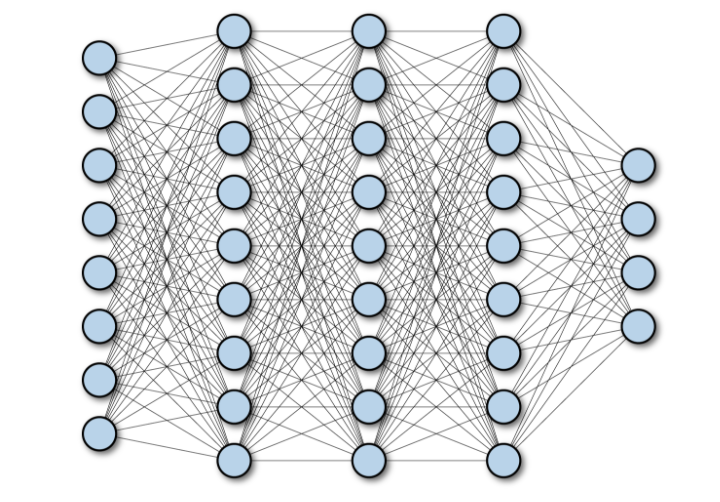
\includegraphics[width=0.50\textwidth]{figures/fully connected}
\caption{Fully Connected Layer semantics~\cite{article}}
\label{fig:fullconn}
\end{figure}


\subsubsection{Sampling layers}\label{subsub:sampling-layers}
Sampling layers are utilised to reduce the spatial dimensions of input data while maintaining its essential characteristics.
This process encompasses techniques such as sub-sampling,
strided convolutions, and global pooling.
The following section provides an in-depth examination of several frequently employed sampling methods.

In the following paragraphs I will discuss some of the most important sampling layers.

\paragraph{Max Pooling}
is one of the most prevalent sub-sampling techniques employed in convolutional neural networks.
In this approach, a sliding window processes the input feature map, and for each window,
the maximum value is selected. This operation reduces the dimensionality of the feature map,
preserving the most notable features (such as edges or textures) while discarding those of lesser relevance.
Max pooling is particularly effective in object detection tasks where maintaining the strongest activations is of paramount importance, as evidenced by the findings of GU.~\cite{GU2018354}.

\paragraph{Average Pooling}
, similarly to maximum pooling, average pooling utilises a sliding window; however, rather than
calculating the maximum value, it computes the average. This results in a more gradual
representation of the feature map and is frequently employed when the objective is to generalise
features to a greater extent than preserving sharp edges~\cite{GU2018354}.


\paragraph{Global Pooling}
methods, such as global max pooling and global average pooling, condense the entire feature map into a single value for each channel,
based on the method chosen, e.g. if the global max pooling is chosen, entire channel is condensed into the maximal value of the channel.
This technique is commonly employed at the conclusion of a convolutional neural network, particularly in image classification tasks, where the spatial location of features is of lesser consequence than their mere presence. Global pooling mitigates the risk of overfitting by producing a compact representation of the input data, as evidenced by Ruby (2020).~\cite{GU2018354}.


\begin{figure}[h]
\centering
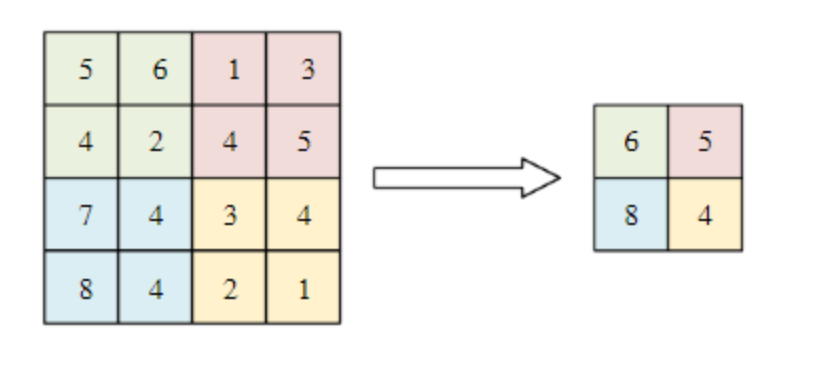
\includegraphics[width=.50\textwidth]{figures/pooling}
\caption{Pooling layer operation~\cite{article}}
\label{fig:pooling}
\end{figure}



\subsubsection{Activation Functions}\label{subsec:activation-functions}

Activation functions are employed in convolutional neural networks and other neural networks to introduce non-linearity into the model,
thereby enabling it to learn complex patterns and relationships within the data by determining the output of each neuron based on its input.
After calculating the weighted sum of the inputs to a neuron, the activation function transforms this sum into the output. These functions allows the model to represent a wide range of functions.
The output of the activation function serves as the input to the next layer.

In light of the work conducted by Siddharth Sharma and Simone Sharma regarding  activation functions~\cite{sharma2017activation}
the most prevalent  activation functions are ReLU, Sigmoid, and Tanh (Hyperbolic tangent).
Although alternative activation functions, such as BSF and ELU, could be employed, they are not utilised by the examined model (Yolov8).
Consequently, a detailed discussion of these functions will not be provided.
The following paragraphs  will discuss the ReLU, Sigmoid, and Tanh activation functions based on the work of Siddharth and Simone Sharma~\cite{sharma2017activation}.


\begin{figure}[h!]
    \centering


    \begin{subfigure}[b]{0.5\textwidth}
        \centering
        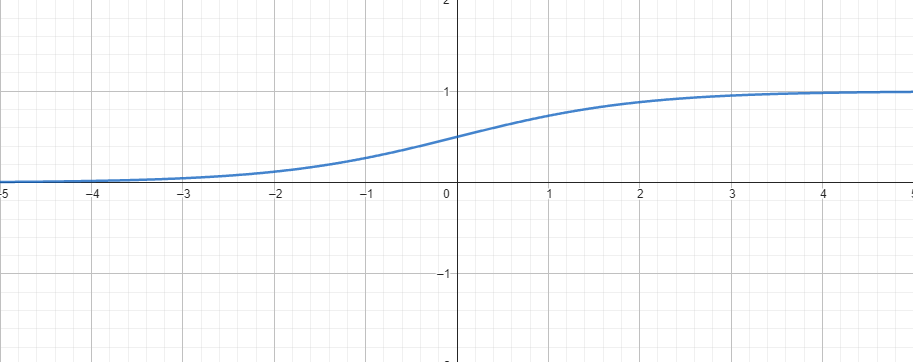
\includegraphics[width=\textwidth]{figures/sigmoid}
        \caption{Sigmoid activation function}
        \label{fig:sigmoid}
    \end{subfigure}
    \hfill
    \begin{subfigure}[b]{0.45\textwidth}
        \centering
        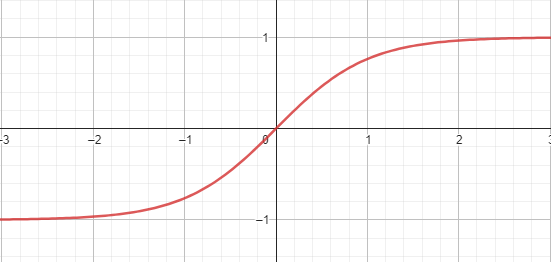
\includegraphics[width=\textwidth]{figures/tanh}
        \caption{Tanh activation function}
        \label{fig:tanh}
    \end{subfigure}
    \hfill
    \begin{subfigure}[b]{0.6\textwidth}
        \centering
        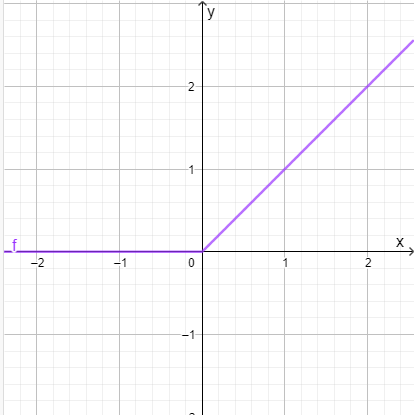
\includegraphics[width=0.5\linewidth]{figures/normal_relu}
        %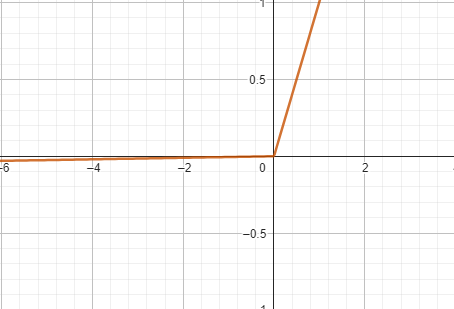
\includegraphics[width=\textwidth]{figures/relu}
        \caption{ReLU activation function}
        \label{fig:relu}
    \end{subfigure}
    \caption{Activation functions: Sigmoid, Tanh and ReLU}
    \label{fig:activation_functions}
\end{figure}


\paragraph{ReLU:}\label{par:relu}
the Rectified Linear Unit (ReLU) is one of the most common and easy to understand activation functions in convolutional (or any other) neural networks.
It is defined as \( f(x) = \max(0, x) \) in the works of Siddharth Sharma~\cite{sharma2017activation}.

This function introduces non-linearity while maintaining a simple and efficient computation.
The ReLU function helps mitigate the vanishing gradient issue, allowing models to learn faster and perform better.

However, be susceptible to the phenomenon known as the \("\)dying ReLU\("\) problem, where neurons become inactive and only output zeros,
particularly during the training of deep networks.



\paragraph{Sigmoid:}\label{par:sigmoid}
the Sigmoid function translates input values to a range between 0 and 1,
rendering it useful for binary classification problems.
It is defined as \( f(x) = \frac{1}{1 + e^{-x}} \) in the works of Siddharth Sharma~\cite{sharma2017activation}.

While the Sigmoid function provides smooth gradients,
it is prone to the vanishing gradient problem,
especially for large positive or negative input values.

This can slow down the training of deep networks,
which is why it is often replaced by other activation
functions in hidden layers,
though it still finds use in the output layer for binary classification tasks.



\paragraph{Tanh:}\label{par:tanh}
the hyperbolic tangent (Tanh) function is another activation function that maps input values to a range between -1 and 1.
It is defined as  \( f(x) = \frac{e^x - e^{-x}}{e^x + e^{-x}} \)in the works of Siddharth Sharma~\cite{sharma2017activation}.

The Tanh function is zero-centered and centrically symmetrical, facilitates the centring of the data and may result in accelerated convergence during training.

Nevertheless, it continues to exhibit the vanishing gradient problem for large input values, though to a lesser extent than the Sigmoid function.



\subsection{Introduction to YOLO}\label{subsec:introduction-to-yolo}

The YOLO (You Only Look Once) model is a relatively recent object detection system that is straightforward to utilise and comprehend, while also benefiting from a thriving community of users and developers.
It is based on the YOLO algorithm, which is a real-time object detection algorithm developed by Joseph Redmon and Ali Farhadi in 2015\cite{redmon2016lookonceunifiedrealtime}.



Unlike traditional object detection methods that apply classifiers to various sections of an image,
YOLO (You Only Look Once) approaches the problem as a single regression problem.
The algorithm divides the input image into an
\(S \times S\) grid and predicts bounding boxes and class probabilities in parallel for each grid cell,
enabling the model to detect multiple types and instances of objects in a single run.
This kind of architecture not only enhances speed by processing the entire image at once
but also improves detection accuracy by reducing the number of false positives.
By minimizing redundant detections and effectively capturing the spatial context of objects,
YOLO allows for real-time applications, given its fast inference speeds, making it particularly effective in scenarios such as video surveillance, autonomous driving, and robotics.

The YOLO model has evolved through multiple versions, with improvements in both performance and varying capability.
Subsequent versions of the model, including Yolov2, Yolov3, and the latest Yolov5 and Yolov7, as well as Yolov8 (with Yolov10 and 11 forthcoming),
have introduced advancements in network architecture,
feature extraction, and training techniques.
These developments have rendered YOLO a suitable candidate for a number of applications,
including autonomous vehicles, as evidenced by my own observations during my work in the industry, surveillance systems, and real-time video analysis.

A further noteworthy attribute of the Yolo-type neural networks is their scalability and versatility in terms of model architecture.
These models are available in a range of sizes (\textit{nano, small, medium, large, extralarge}) and with a variety of detection types (\textit{semantic segmentation, bounding boxes,
oriented bounding boxes, instance segmentation}), which can be deployed in diverse scenarios.




\begin{figure}[ht]
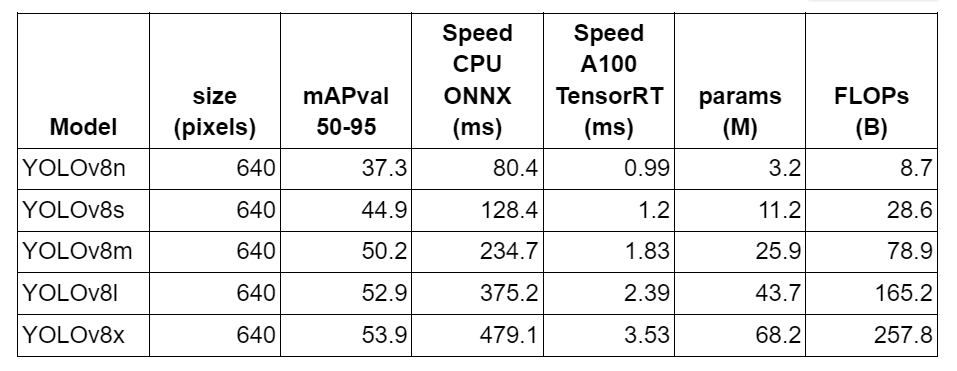
\includegraphics[width=1.0\textwidth]{figures/table1}
\caption{Different sizes of the Yolov8~\cite{githubGitHubUltralyticsultralytics}}
\label{fig:tableofsizes}
\end{figure}
\newpage
\subsubsection{The role of model size}\label{subsubsec:model-size}
In the field of computer vision, particularly in the context of object detection tasks, the selection of an appropriate size for a
Yolov8 model, such as Yolov8-Nano, Yolov8-Small,Yolov8-Medium,  Yolov8-Large, or Yolov8-eXtra-large is of paramount importance in order to achieve an optimal balance between accuracy, speed, and resource efficiency.

The smaller models are lightweight and operate at high speeds, rendering them optimal for real-time applications on devices with constrained computational capabiliti\-es, such as mobile phones or edge devices.
Although they consume less memory and processing power, they may compromise some accuracy, which can be an ac\-cept\-ab\-le trade-off in applications where speed is more important than precision.

In contrast, larger models demonstrate superior accuracy and are capable of handling intricate image details with greater precision, through the models large number of trainable and frozen(not trainable) parameters.
They are better suited to scenarios where there are fewer computational constraints, such as high-powered GPUs or cloud environments, where precise detection is essential.

Selecting an appropriate model size allows developers to tailor solutions to the specific needs of their applications, ensuring both cost-effectiveness and reliability.
This careful selection directly influences the efficiency and effectiveness of computer vision systems, optimising them for diverse deployment environments.

In light of these considerations, I have opted to utilise a medium-sized model, aiming to strike a balance between computational capacity and accuracy.
\newpage
\subsection{Model architecture}\label{subsec:architecture}
This network, like many others in the CNN family, has a distinctive architectural configuration that
enables the execution of intricate tasks such as object detection and classification.
The system is constituted of three distinct and discrete components,
each comprising a unique set of layers that perform specific and separate functions.
The following paragraphs aim to provide an overview of these elements and their contribution to the model's detection.

\begin{figure}[ht]
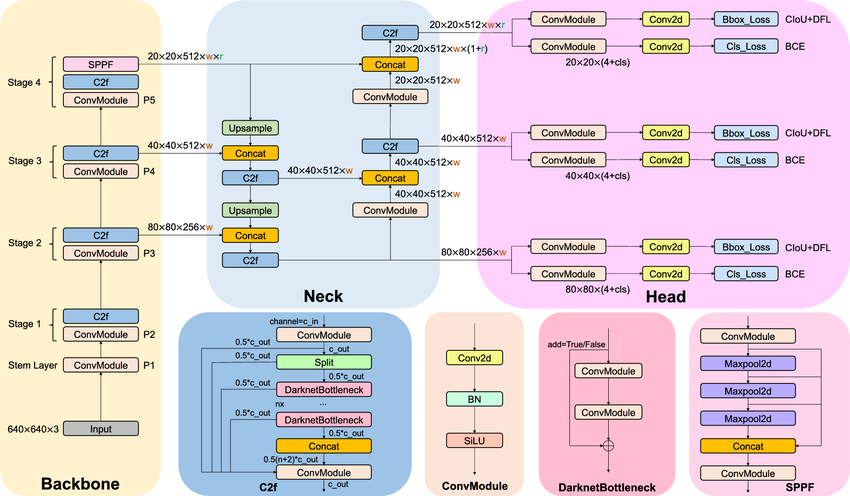
\includegraphics[width=1.0\textwidth]{figures/Detailed-illustration-of-YOLOv8-model-architecture-The-Backbone-Neck-and-Head-are-the}
\caption{The architecture of the Yolov8 model~\cite{FractureDetection2024}}
\label{fig:architecture}
\end{figure}
\paragraph{Backbone:}\label{par:backbone}
the Yolov8 model is based on convolutional neural networks that have been specifically designed to capture essential features from input images.
It comp-ri-ses multiple layers of convolutional operations (called Conv and a complex layer called C2F)
that extract progressively more sophisticated representations.
This structure emphasises both depth and computational efficiency,
enabling the model to discern subtle details while maintaining rapid processing capabilities.
Innovations such as skip connections and normalization techniques are employed to enhance the learning dynamics and improve the model's robustness to variations in input conditions.
%kép a backbone-ról

\paragraph{Neck:}\label{par:neck}
in the Yolov8 architectural design, the neck serves as an intermediary between the backbone and the head.
The primary function of the neck is to consolidate features from the various levels of the backbone,
thereby enhancing the model's ability to detect objects across different scales.
By employing strategies such as feature fusion or pyramid pooling,
the neck effectively integrates both coarse and fine features,
enabling the model to better handle overlapping objects and diverse scene contexts.
This feature aggregation is crucial for optimising the detection performance,
as it allows the model to harness a comprehensive range of information.


\paragraph{Head:}\label{par:head}
the head of the Yolov8 model is responsible for generating the final outputs,
which are based on the features that have been processed through the neck.
The final stage of the Yolov8 model translates the aggregated feature maps into bounding box predictions and associated class scores for each detected object.
This section typically employs a combination of convolutional and fully connected layers to refine these outputs,
ensuring they are accurate and meaningful.
Additionally, the head may implement techniques such as adaptive anchors or
confidence scoring to enhance the localisation and classification accuracy.
By effectively synthesising the rich feature information, the head enables Yolov8 to achieve high-performance object detection suitable for a wide array of applications.

%kép a headről
\subsection{Training}\label{subsec:training}
The training process~\cite{redmon2016lookonceunifiedrealtime} for the Yolov8 model involves feeding its input with a large dataset of labelled images.
The model learns to identify objects by minimizing the difference between its predictions and the actual labels trough multiple iterations:
After a training cycle, if the default settings are kept, a validation function (so called \("\)val\("\))\ is run,
to determine more information on the model's performance on pictures that are not present in the training set.
The training process is iterative, with the model adjusting its parameters to improve its predictions over time.
This process is computationally intensive and requires access to powerful hardware,
the best fitting hardware for this purpose, which can be found in an ordinary PC, is the GPU\@.

The training process involves several key steps, including data preprocessing, model initialization,
loss calculation, and parameter optimization.
The model is trained using a technique called backpropagation, which involves adjusting the model's weights based on
the error between its predictions and the ground truth labels.

The Yolov8 model uses a number of different loss functions, according to the original paper~\cite{redmon2016lookonceunifiedrealtime}
, loss functions to measure the difference between its predictions and the actual labels in different ways:
\newpage


\begin{itemize}
\item \textbf{CIoU (Complete Intersection over Union) loss}:
\begin{equation}
\text{CIoU} = 1 - \left( \text{IoU} - \frac{\rho^2(\mathbf{b}, \mathbf{b}^g)}{c^2} - \alpha v \right) ~\cite{li2020generalizedfocallosslearning}\label{eq:equation3}
\end{equation}
where \(\rho\) is the Euclidean distance between the centre-points of the predicted box \(\mathbf{b}\) and
 the ground truth box \(\mathbf{b}^g\), \(c\) is the diagonal length of the smallest enclosing box covering
 the two boxes, \(\alpha\) is a positive trade-off parameter that serves to balance the importance of the aspect ratio consistency term \(v\),  that measures the consistency of aspect
 ratios.
 It is more sensible to localisation accuracy.

\item \textbf{DFL (Distribution Focal Loss)}:
\begin{equation}
\text{DFL} = -\sum_{i=1}^{N} p_i \log(q_i)~\cite{DBLP:journals/corr/abs-1911-08287}\label{eq:equation2}
\end{equation}
where \(p_i\) is the true probability distribution and \(q_i\) is the predicted probability distribution.
It is sensible to the accuracy classification.
\item \textbf{BCE (binary cross-entropy for classification loss)}:
\begin{equation}
\text{BCE} = -\sum_{i=1}^{N} y_i \log(p_i) + (1 - y_i) \log(1 - p_i)~\cite{ruby2020binary}\label{eq:equation}
\end{equation}
where \(y_i\) is the true label and \(p_i\) is the predicted probability.

\end{itemize}



I opted for training the model on my local machine, using a single GPU, while it provided me with sufficient performance, the training time was significantly longer than it would have been on a more powerful cloud machine.
To reduce the chance of overfitting, the training dataset is typically divided into training and validation sets,
with the latter used to evaluate the model's performance on unseen data.
The trainings batch size where set to 3, which is not common, but it was necessary to fit the model on the GPU,
to optimise training time.

\newpage

%\section[Chosen model, training and data management]{The Model, its training and data management} \label{sec:model-training-data}


%Models for object detection

\section{Object detection component implementation}\label{sec:object-detection-component-implementation}

\subsection{Dataset and formats}\label{subsec:dataset-and-formats}
My project started with choosing and downloading a suitable dataset containing data from urban traffic scenarios.
I chose the Cityscapes dataset~\cite{Cordts2016Cityscapes}.

These data was not in the correct format for the Yolo model to use.
The dataset contains semantic segmentations, but the vanilla Yolo architecture is working with bounding boxes.
I needed to write a format conversion script, following the descriptions in subsection \ref{subsec:data-management}.


\subsubsection{Cityscapes overview}\label{subsubsec:cityscapes}
The Cityscapes dataset is a large-scale dataset~\cite{Cordts2016Cityscapes} used for training and evaluating object detection models.
It contains high-resolution images of urban scenes, with detailed annotations for various objects such as cars,
pedestrians, and traffic signs.
The dataset is widely used in the field of computer vision for tasks such as semantic segmentation and object detection.


I chose the gtFine dataset, consists of precisely labelled segmentation masks.
Based on their work, where they published this dataset~\cite{Cordts2016Cityscapes} titled \("\)\textit{The cityscapes dataset for semantic urban scene understanding}\("\)
the gtFine dataset consists of 5000 images,
with a resolution of 1024\(\times\)2048 pixels, and annotations for 30 classes of objects.
It is divided into three subsets: training set, validation set, and test set, with 2975, 500, and 1525 images, respectively.

The validation and training sets contain annotations for 30 classes, while the test set does not include any annotations.
The dataset is labelled using pixel-level segmentation masks, which provide detailed information about the
location and shape of objects in the scene.

However, for the purpose of this work, the annotations were converted into a bounding-box format,
which is more suitable and straightforward for this object detection tasks.
Also, the dataset was filtered to include only the classes that are relevant to the project.

\subsection{Data engineering} \label{subsec:data-management}
The images and annotations are converted to a format that the Yolov8 model can process, which is
a text file that contains the path of the image and the coordinates of the bounding boxes in pixels for each object in the image.
The format is straightforward: each line of the text file represents a single instance of an object.
The first variable is the label\_id, which denotes the object's class.
This is followed by the two-point's four \((x, y)\) type coordinates in pixel.
This process uses a custom script that reads the annotations from the Cityscapes dataset and converts the labels
into labels whose classes are filtered and transformed the relevant classes into the grouping I chose for this project.

The classes were grouped into five categories:
\begin{itemize}
    \item \textbf{small vehicle}~\textit{(usually cars, which are for personal use)},
    \item \textbf{large vehicle}~\textit{(buses, trucks and other large non personal vehicles)},
    \item \textbf{two wheeler}~\textit{(bicycles and motorcycles)},
    \item \textbf{On-rails}~\textit{(trains and trams though the smaller Fine dataset did not include any in the training set)}
    \item and \textbf{person}~\textit{(pedestrian, and rider)}.
\end{itemize}

The categories were selected on the basis that the model's confusion is more readily managed when objects
that are more similar in appearance are grouped together, thereby facilitating the model's ability to
distinguish between them.

The script also converts the semantic segmentation masks into bounding boxes, trough finding the most
extreme points and of the mask, creating a bounding box around them.
This converted output is then saved into a text file, which is in the format used as input for the Yolov8 model.

The final structure of the dataset with metadata (descriptors and lists of labels and pictures) is as follows:
\begin{itemize}
    \item \textbf{Root (gtFine)}: The root directory of the Cityscapes dataset, which contains the images and annotations.
    \begin{itemize}
        \item \textbf{image}: Folder containing the images in the dataset, broken down into training, validation, and test sets
    and further divided into subfolders based on the city where the images were captured.
        \item \textbf{labels}: The class label for each object in the image, with the same subfolder structure as the images.
        \item \textbf{train.txt}: The training set, which contains the paths to the training images and their corresponding annotations.
        \item \textbf{val.txt}: The validation set, which contains the paths to the validation images and their corresponding annotations.
        \item \textbf{test.txt}: The test set, which contains the paths to the test images and their corresponding annotations.
    \end{itemize}
    \item \textbf{Descriptors}: The folder containing a list of class labels and their corresponding indices, as well as
    path set descriptor txt-s, the train-, val- and test.txts.
    It is used by the model to determine the classes, their indices and the paths to the images.
\end{itemize}


\subsection{Model Implementation}\label{subsec:model-implementation}


\subsubsection{Justification behind the selection of YoloV8}\label{subsubsec:justification-behind-the-selection-of-yolov8}


For my work, I chose the~\textbf{Yolov8m} configuration, which stands for \textbf{Yolo version 8 medium}.
My choice was made on the bases of previous experience with this model architecture and the popularity of its applications,
made it so there are an abundance of literature regarding this specific algorithm and architecture.
It is also suitable for numerous, different applications, this aspect was important because of the high variance in sizes and shapes of the traffic objects needed to be detected by the network.
Training with custom datasets has also been made relatively easy.

I also examined other networks such as Faster R-CNN and even an older Yolo version, Yolov5.
I tested Yolov5 on the same dataset and produced inferior performance KPIs (Key Performance Indicators).
I confirmed my findings by a paper that was discussing an application of these models~\cite{Chitraningrum_Banowati_Herdiana_Mulyati_Sakti_Fudholi_Saputra_Farishi_Muchtar_Andria_2024},
Yolov5 exhibits inferior performance relative to Yolov8 on identical input data and with an equivalent architectural configuration.
Additionally, it is also faster.
This comparison renders the Yolov5 model obsolete, and therefore it has been excluded from further consideration.

The Faster R-CNN while being a less sophisticated model it gets outperformed by Yolo on,
a comparison study on these networks \("\)Analysis of the performance of Faster R-CNN and Yolov8 in detecting fishing vessels and fishes in real time\("\)~\cite{ezzeddini2024fishing}
it has a table which contains all the necessary information to decide that it is inferior to Yolov8 in almost every aspect, thus it was not chosen over the Yolo architecture.

Given its superior performance compared with the two models examined
as well as the extensive availability of related materials, and it's ability to predict bounding boxes and class
probabilities for objects in an image, the Yolov8 algorithm has been selected for this undertaking.

\subsubsection{Chosen model's description and parametrisation}\label{subsubsec:model-architecture}

Based on paragraph~\ref{subsubsec:justification-behind-the-selection-of-yolov8} the Yolov8 bounding box
detection medium version of the model was picked for this project.
In order to facilitate the requirements of the project, the model was utilised in a pre-trained state,
with the weights being downloaded from the official Yolov8 repository~\cite{githubGitHubUltralyticsultralytics}, trained on the COCO dataset, as described in the paper where they introduced the network~\cite{redmon2016lookonceunifiedrealtime}.
Subsequently, the model was fine-tuned on the Cityscapes dataset, which was converted into a format compatible with the model's processing capabilities.

Training was conducted using the Adam optimiser with a learning rate of 0.01 for lr1 (initial learning rate) and lrf (final learning rate).
I ran the training on the model for 30 epochs with a batch size of 3, to accommodate the limited local GPU memory.
The training process ran on a single PNY NVIDIA Quadro P2000 5GB VCQP2000-PB GPU, with a total training time of 28.056 hours.

\subsubsection{Training with the help of MLOps solutions}\label{subsec:training-with-the-help-of-mlops-solutions}
In order to monitor the performance of the model and to facilitate the visualisation of the learning process,
as well as to organise the experiments, an online machine learning monitoring solution, Comet.ml, has been selected.

This tool is capable of tracking the training process in real time and of visualising the properties of the model on
a user-friendly dashboard, which can be accessed from any device with an internet connection.
The Comet.ml platform also provides a range of features that can be used to compare different experiments,
such as hyper-parameter tuning, model versioning, and collaboration tools, while also offering a comprehensive
set of APIs for integration with other tools and platforms.

\begin{figure}[ht]
\centering
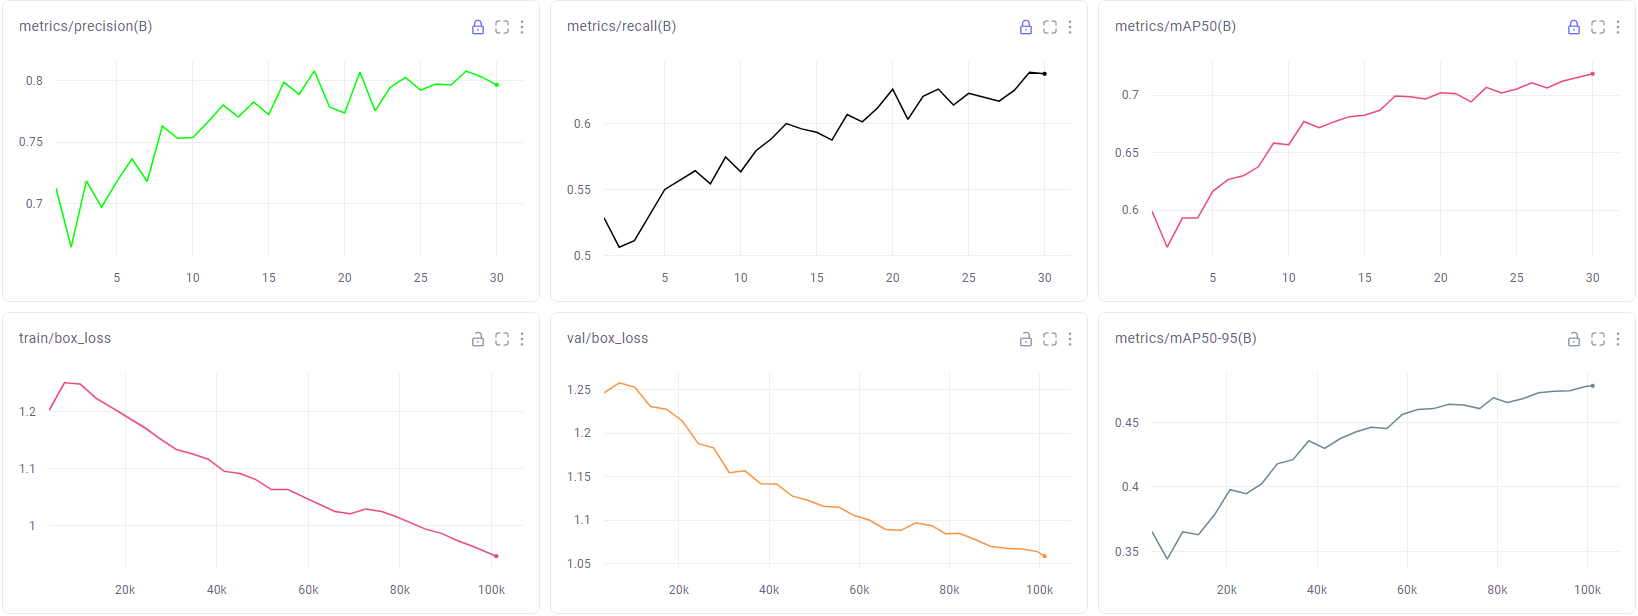
\includegraphics[width=1.0\textwidth]{figures/model}
\caption{Comet.ml dashboard made from the training of our model.}
\label{fig:comet}
\end{figure}

Figure~\ref{fig:comet} depicts the Comet.ml dashboard, which offers a comprehensive representation of the training process,
encompassing loss and accuracy metrics, the learning rate, and the model's performance on the validation set.
This information is vital for evaluating the model's performance and for identifying potential issues that may arise during training.

Furthermore, the Comet.ml platform enables the comparison of different experiments,
which can be beneficial for fine-tuning the model's hyperparameters and for improving its performance.
Which I did try out, for comparing the performances of the same model on the same dataset,
but with different epochs and batch sizes to see and find a good balance between training time and performance.

\subsubsection{Model evaluation}\label{subsubsec:model-evaluation}
The evaluation of the Yolov8 model is performed using a set of metrics that measure its performance on the Cityscapes dataset.
These metrics include precision, recall, mAP, and IoU, which are commonly used in object detection tasks.
I used the mAP metric to evaluate the model's performance on the test set, which provides a comprehensive measure of its accuracy.
The mAP is calculated by averaging the precision-recall curves for each class in the dataset, which gives an overall measure of the model's performance.

\begin{equation}
\text{mAP} = \frac{1}{N} \sum_{i=1}^{N} \text{AP}_i
\end{equation}


where \( N \) is the number of classes and \( \text{AP}_i \) is the average precision for class \( i \).

The IoU metric is used to evaluate the model's ability to accurately predict the bounding boxes for objects in the image.
It measures the overlap between the predicted and ground truth bounding boxes, with a higher IoU indicating a more accurate prediction.

\begin{equation}
\text{IoU} = \frac{\text{Area of Overlap}}{\text{Area of Union}}
\end{equation}


In order to ensure the reliability of the subsequent analysis, only those detections with an IoU value of at least 0.80 were considered,
and only those predictions with a relatively high degree of accuracy were utilised.

The performance of the final and best performing model (which will be later used in the interpretation generating component) is evaluated on the test set's all classes averaged:


\begin{table}[h!]
\centering
\begin{tabular}{|c|c|c|c|c|c|c|}
\hline
\textbf{Class} & \textbf{Images} & \textbf{Instances} & \textbf{Box(P} & \textbf{R} & \textbf{mAP@0.5} & \textbf{mAP@0.5:0.95)} \\
\hline
all            & 500             & 10654             & 0.797           & 0.638      & 0.719            & 0.478                 \\
small\_vehicle & 479             & 4832              & 0.889           & 0.751      & 0.834            & 0.604                 \\
person         & 441             & 4095              & 0.829           & 0.651      & 0.738            & 0.445                 \\
large\_vehicle & 141             & 191               & 0.729           & 0.597      & 0.666            & 0.511                 \\
two-wheeler    & 361             & 1536              & 0.741           & 0.553      & 0.637            & 0.354                 \\
\hline
\end{tabular}
\caption{Network performance is evaluated across all classes, considering a detection valid if it achieves an IOU (Intersection Over Union) of at least 70\%.}
\label{table:performance_metrics}
\end{table}



%Szerintem ide kéne tenni aka tanításos elméleti részról a bekezdés utánna meg a MLOps os részt




%----------------------------------------------------------------------------------------%

%! Author = NyPeter
%! Date = 2024. 10. 13.

\section{Model Interpretation}\label{sec:model-interpretation}

\subsection{Importance of Interpretation}\label{subsec:importance-of-interpretation}

Interpreting machine learning models is essential for understanding their decision-making processes.
It helps in identifying biases, improving model performance by providing information helping us the augment data more efficiently, and building trust with users.
Interpretation techniques provide insights into how image processing models make predictions and highlight the most influential features.

Interpretation of machine learning algorithms is a fairly new field, but it has gained significant attention
in recent years due to the increasing complexity of models and the need for transparency and accountability.
This need comes form industrial and judicial actors, who require explanations for the decisions made by models,
especially in safety-critical applications such as autonomous vehicles, healthcare, and finance.
In the last couple of years, the field of model interpretation has seen significant advancements, each brought
us closer to understanding the inner workings of machine learning models, and try to put reason and logic behind
otherwise black-box models.

Furthermore, based on these advancements the aforementioned actors are more willing to adopt laws,
standards and regulations that require models to be interpretable,
if they are to be used in non-research areas.

Building on the aforementioned state of the machine learning world, I felt it was important to try
and create a fairly coherent interpretation of the model to meet today's industry standards.

\subsection{Introduction to Interpretation methods}\label{subsec:introduction-to-interpretation-methods}

Model interpretation is a critical aspect of machine learning that aims to explain the decision-making process of models. % Ismétlés
Interpretable models are essential for building trust with users, identifying biases, and with this information,
developers have a deeper understanding that can help them improve model performance.
In this section, there will be a discussion of the importance of model interpretation and a review of different methods of interpretation.

In their survey~\cite{LIANG2021168}, Liang et al. highlight the significance of model interpretation techniques in providing insights from the model itself, and the output of the model, without knowing the inner state of the model.

Therefore they sorted these techniques into two categories:
\begin{enumerate}
    \item data driven or more commonly as model-agnostic methods
    \item model driven or model-specific methods
\end{enumerate}

The following sections will provide an overview of the two categories.
In the event that one is used, an analysis of the algorithms will be presented in light of the implementation used in this project.
This will include a comparison and contrast of their respective strengths and weaknesses.



\subsection{Model-Agnostic Methods}\label{subsec:model-agnostic-methods}
Based on the work of  Liang~\cite{LIANG2021168}, model-agnostic interpretation methods can be divided into three categories:
\begin{enumerate}
    \item Perturbation-based interpretation and a Game theoretic approach
    \item Adversarial-based interpretation
    \item Concept-based interpretation
\end{enumerate}


As discussed in the work of Liang~\cite{LIANG2021168}, these are designed to explain model predictions without relying
on the internal structure of the model hence their name, making them applicable to a wide range of models.
This insight may be more applicable to local examples, as the approach only provides explanations for the given data and not globally for the model itself.
For image processing purposes, these methods are particularly easy to understand and implement.

Both the game-theoretic and perturbation-based interpretation methods involve altering the input data
and observing the resulting changes in the predictions of the model on the modified image, while Adversarial-based interpretation methods focus on generating small perturbations or adversarial examples that can significantly change the predictions, highlighting the model's vulnerabilities.

On the other hand, concept-based interpretation methods aim to link model behavior to high-level human-understandable concepts.

Regardless, I will discuss the different types of data-driven interpretation methods in the following paragraphs, each on the basis of Liang's work~\cite{LIANG2021168}

\subsubsection{Perturbation-based Interpretation}\label{subsubsec:pertubation-based-interpretation}

Perturbation-based interpretation methods are model-agnostic techniques that explain model predictions by perturbing the input data.
These methods generate perturbed samples by introducing noise (or masking portions of the image) to the input image and observing the alterations in the model's predictions.
This masking is the main principle behind these methods.

The most common type of masking is occlusion, where parts of the image are covered to determine their importance for the model's output.
It can be interpreted as a form of feature selection, where the model's output is evaluated based on the presence or absence of specific features.

In essence, perturbation-based methods can be conceptualised as an optimisation problem.
Given an input vector \( x \), a model function \( f(x) \), and a predicted vector \( y \),
the objective is to identify which components of \( x \) contribute to the generation of the prediction. To accomplish this, the input features are systematically altered by introducing perturbations \( \delta x \)).
This approach allows us to infer the importance of specific features by quantifying the extent to which the predicted vector \( f(x + \delta x) \).
This approach allows us to infer the importance of specific features by quantifying the extent to which the predicted vector y is affected by the introduction of these perturbations.



Perturbation-based methods are focusing on \("local\) \(interpretability"\), meaning they explain specific predictions rather than providing an overarching understanding of the model’s behaviour.
This local explanation is vastly inferior to global interpretability.
Regardless, sometimes it can be extended, to provide broader insights into the models logic.

It works in a similar way to the human visual system and the way we perceive the visual world,
so that by obscuring different parts of an object, we can significantly alter our own eye's perception of the object.
By analysing the effect of perturbations on the model's output, these methods identify the most important features for a given prediction.

As a prominent implementation of this method is LIME (Local Interpretable Model-agnostic Explanations), which will be discussed in a following section section~\ref{subsec:methods-for-model-interpretation}, it was selected
for use in the project due to its simplicity and effectiveness in interpreting the model's predictions.


There are multiple types of perturbations:
\begin{itemize}
    \item \textbf{Noise insertion}: adding some type of noise (Gaussian or random) to parts of the input data.
    which can reveal the sensitivity of the model to small variations.
    \item \textbf{Blurring/Pixel Modification}: when working with image data, perturbations can be created by blurring parts of an image or modifying pixel intensities, which helps to understand how the clarity or sharpness of particular regions affects the prediction.
    \item \textbf{Feature Deletion for structured data}: remove or zeroing specific features, determining how significant that feature really is to the prediction.
    \item \textbf{Text Data Perturbations}: for text data, this involves removing words, phrases, characters, but it can also mean swapping tokens with synonyms to gauge their importance to the output.
\end{itemize}

Given the project's domain, I only used perturbations used in image processing tasks, and these exclusively consists of modifying pixels and groups of pixels to determine their usefulness to the detection.
In the following, I will discuss two variations of this standard perturbation-based approach.

\paragraph{Game theoretic approach with perturbation}\label{par:game-theoretic-approach-with-pertubation}

 is a model-agnostic interpretation method that employs cooperative game theory to explain model predictions.
This translates to decomposition of the input image into a number identical, equally-sized components, referred to as \("\)features\("\).
These are processed further and a so called Shapley value is calculated to each feature, based on their contribution to the prediction.
This will be projected onto the image, where each feature will be coloured according to this value, thus facilitating easier reading and comprehension.
A detailed examination of this process can be found in reference \ref{par:shap}, where the operational mechanics of this methodology will be elucidated.

Based on the work of Lundberg~\cite{lundberg2017unifiedapproachinterpretingmodel} and Liang~\cite{LIANG2021168},
this method, namely SHAP (SHapley Additive exPlanations), is particularly useful for image processing tasks, as it provides detailed insights into the model's decision-making process.
On grounds of the aforementioned, I chose to use SHAP in my project, as it offers a comprehensive and theoretically grounded approach to interpreting the model's predictions.

\paragraph{Adversarial-based interpretation}\label{par:adversarial-based-interpretation}

methods, based on the work of Lian~\cite{LIANG2021168},
represent a subtype of perturbation methods,
the objective of which is to provide more robust interpretations.
These methods address a common issue in deep neural networks (DNNs), namely poor generalisation performance, as highlighted in the base of my work~\cite{LIANG2021168}.
Deep neural networks (DNNs) are highly sensitive to perturbations in input data, which can result in significant alterations to the predictions made,
thus affecting the stability and reliability of the interpretations produced.
The earliest adversarial-based interpretation methods, as exemplified by the approaches put forth by Fong et al. (2017) and other researchers,
employed techniques to mitigate the impact of perturbations.
This was achieved by utilising random masks and regularising the masks with total-variation norms to smoothen the images that had been perturbed.

Although these methods enhance robustness, they necessitate manual tuning of hyperparameters and yield interpretations of relatively low resolution,
thereby constraining their capacity for fine-grained analysis.
On these grounds, they are not suitable for applications that require high-resolution interpretations, and such I did not use them in my project.

\subsubsection{Concept-based Interpretation}\label{subsubsec:concept-based-interpretation}

Concept-based interpretation methods, based on the work of Liang~\cite{LIANG2021168}, employ predefined sets of human-understandable concepts to provide explanations for deep learning models.
The generation of these concepts is typically conducted with the assistance of domain experts, thereby rendering this method particularly
useful for interpreting the decision-making processes of models in a manner that aligns with human intuition.
The process commences with the selection of a concept set (\(C\)), which encompasses images or data that correspond to specific attributes of the input.
For instance, the concept set may include images of tiger stripes for an image of a tiger.

The definition of these concepts is facilitated by humans, and the concept set is subsequently incorporated into the deep neural
network (DNN) in order to ascertain which concepts are most relevant to the model's predictions.
Two prominent concept-based interpretation methods are Testing with Concept Activation Vectors (TCAV) and Network Dissection (ND).
TCAV explains the behaviour of the model in question by employing human-defined concepts, namely Concept Activation Vectors (CAVs)
, which quantify the importance of said concepts to the model's predictions through directional derivatives.
This approach allows for the assessment of the sensitivity of the model's predictions to specific concepts,
such as texture or colour, across a range of inputs.

In contrast, Network Dissection quantifies the relationship between internal neural network features and visual concepts,
utilising metrics such as Intersection over Union (IoU) to ascertain the degree to which individual neurons correspond to
concepts such as colour, texture, or objects. This approach facilitates a comprehensive understanding of the specific layers
and neurons in a CNN that are responsible for detecting various concepts, thereby offering insights into the interpretability of each layer.

Based on the work of Liang~\cite{LIANG2021168}, these methods are particularly useful for image processing tasks,
as they provide human-understandable explanations for the model's predictions.
However, they require the input of domain experts to define the concepts, which can be time-consuming and may introduce bias.
Furthermore, the interpretability of these methods is limited by the quality of the concept set, which may not capture all
the relevant features of the input data.

As a result, I found that these methods were not suitable for my project, as they
require a high level of domain expertise and may not provide the level of interpretability required for fine-grained analysis.





\subsubsection{Comparison of chosen Model-Agnostic Methods}\label{subsubsec:comparison-of-model-agnostic-methods}

In this subsection, I will compare two of the most popular model-agnostic interpretation methods, LIME and SHAP.
Based on the work of Liang~\cite{LIANG2021168}, these model-agnostic interpretation methods have their strengths and weaknesses.
Through their example I will illustrate the differences between the two methods.

LIME and SHAP while using
different approaches, there are both using some form of perturbation to explain the model's predictions.
LIME approximates the model locally by fitting a simple interpretable model around
the prediction of interest, providing local explanations by perturbing the input
data and observing the changes in the model's predictions.
It is generally faster and simpler, making it suitable for quick, local explanations.


On the other hand, SHAP is based on cooperative game theory and uses Shapley values to attribute the contribution of
each feature to the prediction.
It provides both local and global explanations by considering all possible combinations of features,
producing consistent and theoretically sound explanations.


Based on the discussions by~\cite{lundberg2017unifiedapproachinterpretingmodel}, Kernel SHAP, a variant of SHAP,
is particularly useful for image processing tasks, as it can handle high-dimensional data efficiently.
It is based on the idea of approximating the model with LIME and using the Shapley values to explain
the predictions the model made.
This approach combines the strengths of both LIME and SHAP, providing accurate and efficient explanations for
image processing models.

However, SHAP is more computationally intensive due to the necessity of considering all potential feature combinations. During the execution of the interpretation scripts, SHAP exhibited approximately four times the GPU memory usage of LIME, while the runtime was approximately one hundred times longer. While LIME is flexible and can be applied to any model and data type, SHAP offers a more comprehensive and theoretically grounded approach at a higher computational cost.

\subsection{Model-Specific Methods}\label{subsec:model-specific-methods}
The base idea behind this category is to ground our interpretation on the internal state of the model.
By this in the field of image processing, it aims to somehow visualize some parameters of the inner state of the model, and project it back to the input image.
Multiple methods exist in this category, such as Class Activation Maps, Gradient-based methods.
The following paragraph, present a discussion of the Class Activation Maps with reference to the work of Bany Muhammad and his introduction of his interpretation method~\cite{Muhammad_2020}.
Its implementation will be discussed in the next section.
Furthermore, I will discuss the Gradient-based methods based on the work of Selvaraju titled \("\)Grad-CAM: Visual
Explanations from Deep Networks via Gradient-Based Localization\("\)~\cite{Selvaraju_2019}.




\subsubsection{Class Activation Maps}\label{subsubsec:CAM}

Class Activation Maps (CAMs) are a model-specific interpretation method designed to highlight the regions or features
in an image that are most pertinent to a given model.
In an image, these are the regions that are most relevant to a model's decision, particularly in the context of classification tasks.
The operation of CAMs is based on the projection of the activations from the convolutional layers back onto the input image.
This results in the generation of a heatmap, visually represents the areas that contributed
the most to the prediction~\cite{Muhammad_2020}.
This method provides valuable insights into which features the model is focusing on, enabling a better understanding of
the model's decision-making process.

The original CAM technique, first introduced by Zhou et al. (2016),
is specifically designed for models that include global average pooling layers before the final output layer,
often referred to as the \("\)head\("\).
These pooling layers facilitate and are responsible for the smooth projections (feature maps) on the methods output image.
While the CAM technique is highly effective, it is somewhat limited in that it is optimized for this specific architectural
configuration, which restricts its versatility.
It is less flexible for networks that rely on fully connected layers following the convolutional layers~\cite{Zhou_2016}.

To illustrate, in a classification task where a model identifies a vehicle in an image, CAM would generate a heat map over and around the vehicle.
This indicates that the model primarily focused on that object when making its decision, which is a useful insight.
In the absence of this information, there is a possibility that the network may be detecting a feature that is not
exclusive to that particular object class and this can result in greater confusion within the model.

This type of visual feedback is especially valuable in domains such safety critical (automotive, etc.) or medical fields,
where understanding why the model identifies certain patterns is critical~\cite{Muhammad_2020}.

In response to the architectural limitations of the original CAM method, several improvements have been proposed.
One significant extension is Grad-CAM (Gradient-weighted Class Activation Mapping), which eliminates the dependence
on specific model architectures by using gradients to compute the heatmaps.
Details of Grad-CAM will be further discussed in the next section~\cite{Selvaraju_2019}.

\subsubsection{Gradient-based Methods}\label{subsubsec:gradient-based-methods}

Gradient-based methods, such as Grad-CAM (Gradient-weighted Class Activation Mapping),
take a different approach by utilizing the gradients flowing through the backpropagation of
the network. It can be used to localize the features within the image, that the models learn on.
Grad-CAM generates heatmaps that highlight the regions of the image that contributed the most to the model's output.
Selvaraju et al. (2019) demonstrated the effectiveness of this technique in their work titled
\("\)Grad-CAM: Visual Explanations from Deep Networks via Gradient-Based Localization\("\)~\cite{Selvaraju_2019}.

By leveraging gradients, Grad-CAM provides more precise localization of features compared to basic CAM techniques,
making it particularly useful for deep neural networks in image recognition tasks.

At the end, this method, despite of being more accurate than the vanilla EigenCAM, I did not use it in my project due
to two main considerations.

First of all, the method is more computationally expensive, and requires more memory to run.

Secondly, the method is more complex to implement and requires more input from the model's internal state.
In order to ensure the model calculates the gradients correctly, it should be fed with the whole back-propagation chain,
which has made the other interpretation methods more time-consuming to implement and run.

Based on that I chose to use the CAM method in my project, as it is simpler to implement and provides valuable insights into the model's decision-making process.

\newpage
\subsubsection{Comparison of Model-Specific Methods}\label{subsubsec:comparison-of-model-specific-methods}

Both CAM and Grad-CAM methods have been widely adopted for interpreting convolutional neural networks
and are valuable tools for visualizing and understanding model behaviour.
While CAM is limited by its dependence on specific model architectures, Grad-CAM offers a more flexible and
generalizable approach that can be applied to a wide range of models.
The use of gradients in Grad-CAM allows for more precise localization of features within the image,
providing valuable insights into the decision-making process of the model.

In contest of the resulting visualizations, the output of the two networks tends to be really similar to each other.
Which can be because the two methods are based on the same principle, and the implementation of the Grad-CAM
is a direct extension of the CAM method, utilizing the activation maps with the gradients to provide the explanation.

\subsection{Comparison of Interpretation Methods}\label{subsec:evaluation-interpretation-methods}

In this section, I will compare the model-agnostic and model-specific interpretation methods discussed and chosen in the previous subsections
and paragraph.
Model-agnostic and model-specific interpretation methods each offer unique strengths and weaknesses when applied to
an image processing model.
Both approaches aim to provide insights into the model's decision-making.
However, they are fundamentally different in terms of their underlying assumptions, flexibility, and computational requirements.


Model-agnostic methods often operate by perturbing the input data, observing the changes in the  predictions of the model,
and deriving explanations based on these observations as discussed previously~\ref{subsubsec:pertubation-based-interpretation}.
This makes them highly flexible and applicable to a wide variety of tasks and models.
However, this flexibility sometimes comes at the cost of interpretability precision, as model-agnostic methods approximate
how a model behaves based on perturbations, which may not capture the complete depth of the model’s decision logic.

Conversely, model-specific methods are designed to align with the internal mechanisms of a specific model architecture,
thereby facilitating the generation of explanations based on the model's inherent operational logic.
These methods are often more precise, as they can directly access the model's components — such as layers,
weights, activation vectors, or gradients and utilize this information to interpret how the model made its decision.
In fields like image processing, model-specific methods, such as Class Activation Maps (CAMs) or Gradient-based approaches,
provide visual insights into the areas of an image that most influenced the model’s predictions.
By visualizing the internal state of the model, model-specific methods offer a more direct way of understanding the behaviour of the model,
especially in tasks where identifying critical features or regions of the data is essential.

In comparing these two categories, the fundamental difference lies in their generalization versus precision.
Model-agnostic methods are particularly useful because of their ability to work across different models and domains,
making them versatile tools in scenarios where multiple model types and architectures are used.
However, they frequently offer a higher-level view of the behaviour of the model, which may be less precise than the
insights gained from model-specific methods.
Conversely, model-specific methods provide a more detailed data for understanding of the decision-making process,
directly interacting with the internal components.
This allows for more detailed insights but limits the applicability to certain model types.








%! Author = NyPeter
%! Date = 2024. 10. 13.



%\section{Model interpretation using external solutions}\label{sec:model-interpretation-%application}
\section{Model interpretation component}\label{sec:model-interpretation2}

\subsection{Methods for model interpretation}\label{subsec:methods-for-model-interpretation}

\paragraph{EigenCAM}\label{par:eigencam}
EigenCAM is a model-specific interpretation method that visualizes the regions of an image that are most
important for a model's prediction.
It computes the principal components of the feature maps and highlights the areas that contribute the most
to the final decision.

\paragraph{Local Interpretable Model-agnostic Explanations}\label{par:lime}
LIME is a widely used model-agnostic interpretation method that explains individual predictions by
approximating the model locally with an interpretable model.
It perturbs the input data and observes the changes in the model's predictions to identify the most
important features.

\paragraph{Shapley Additive explanations}\label{par:shap}
SHAP is another model-agnostic method that provides consistent and accurate explanations for model predictions.
It is based on cooperative game theory and assigns a Shapley value to each feature,
representing its contribution to the prediction.

%Methods for interpretation: LIME, SHAP
\subsection{Evaluation of interpretation methods}\label{subsec:evaluation-of-interpretation-methods}
%Results on small_vehicle
% Képmagyarázat
% Detekció bizonyossága vs interpretáció zajosság

\subsection{Addressing the Anomaly regarding the noise of SHAP and the probability of the models detection}\label{subsec:Addressing the Anomaly regarding SHAP and the probability of detection}

\section{Results}\label{sec:results}
SHAP:
\begin{figure}[h]
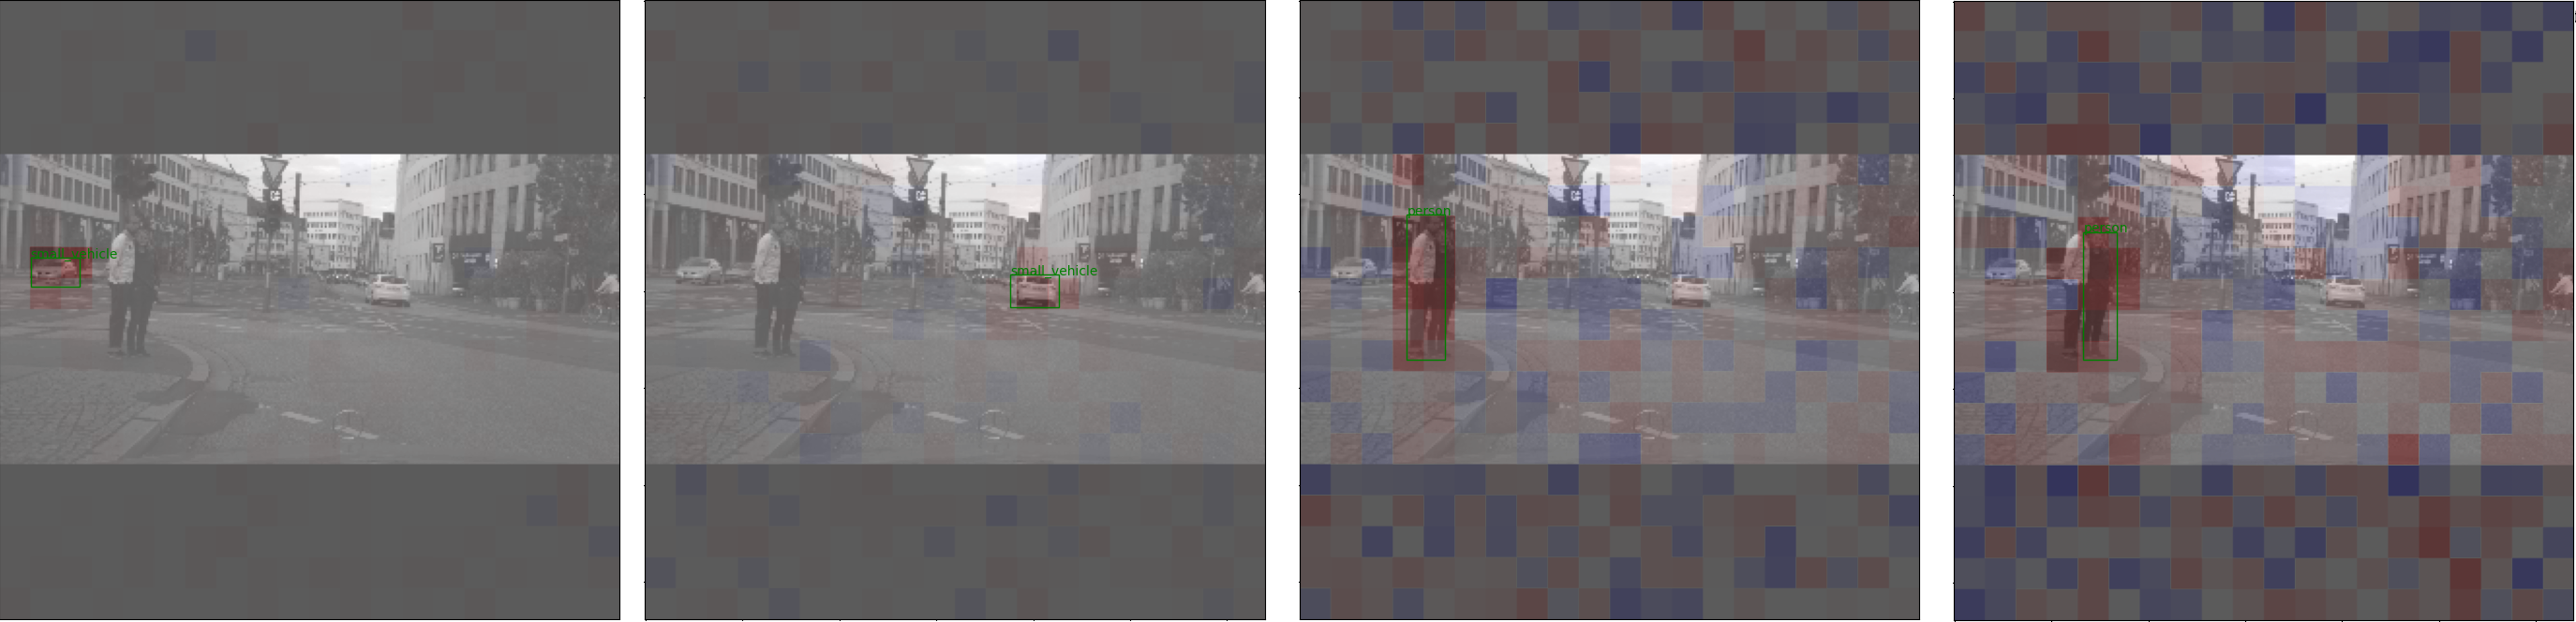
\includegraphics[width=1.0\textwidth]{figures/output1}
\caption{SHAP results for the small vehicle class}\label{fig:SHAP_results1}
\end{figure}
%appliaction of methods


\section{Summary}\label{sec:results}
%appliaction of methods
\begin{figure}[h!]
    \centering
    \begin{subfigure}[b]{\textwidth}
        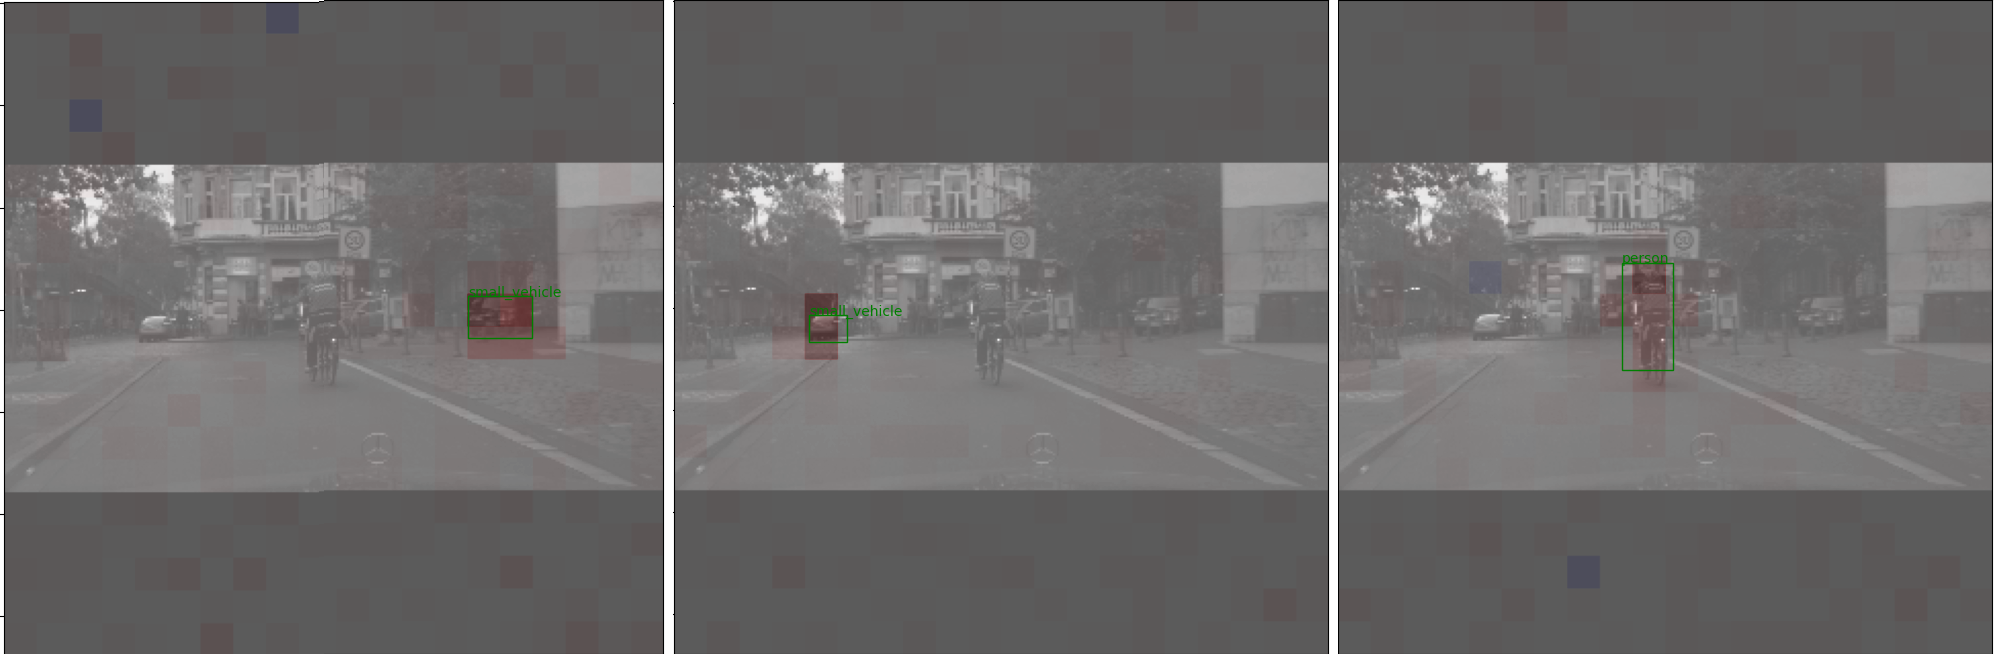
\includegraphics[width=\textwidth]{figures/output}
        \caption{SHAP results}\label{fig:SHAP_results2}
    \end{subfigure}
    \hfill
    \begin{subfigure}[b]{\textwidth}
        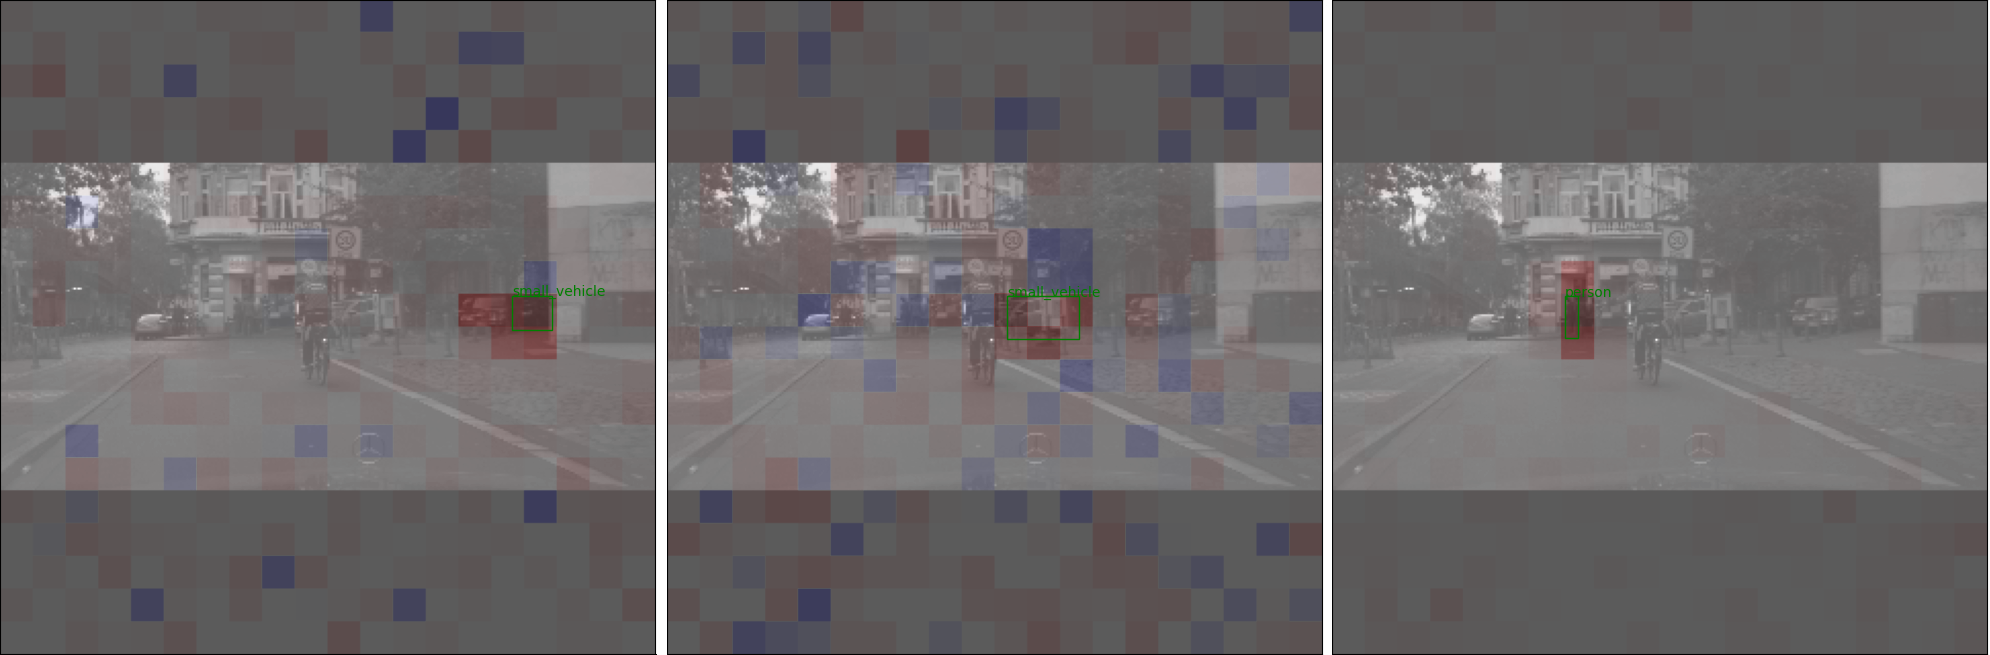
\includegraphics[width=\textwidth]{figures/output2}
        \caption{SHAP results}\label{fig:SHAP_results20}
    \end{subfigure}
    \hfill
    \begin{subfigure}[b]{\textwidth}
        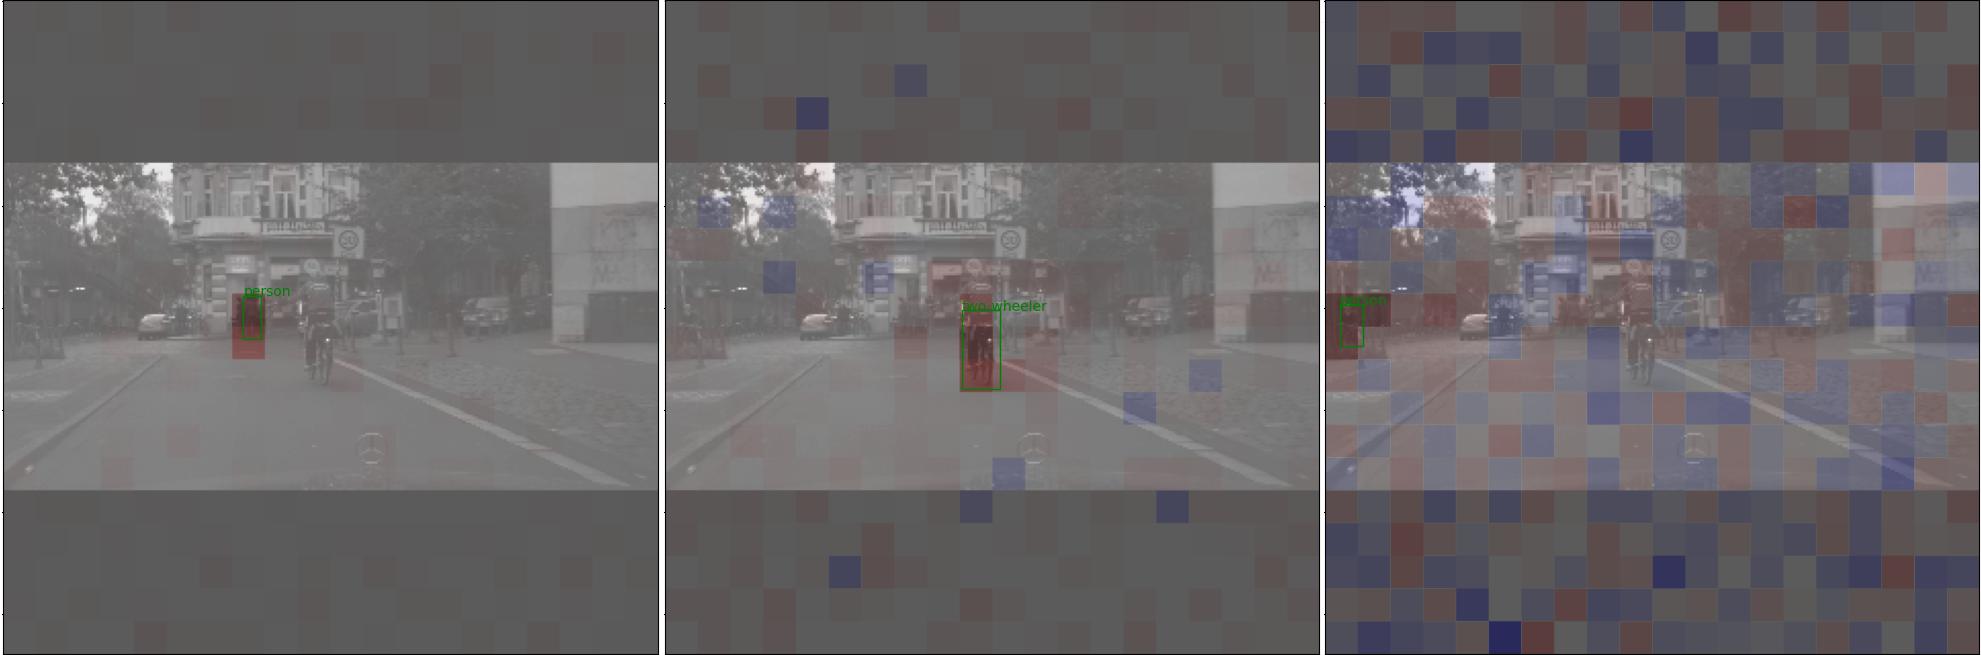
\includegraphics[width=\textwidth]{figures/output2,1}
        \caption{SHAP results}\label{fig:SHAP_results21}
    \end{subfigure}
    \hfill
    \begin{subfigure}[b]{\textwidth}
        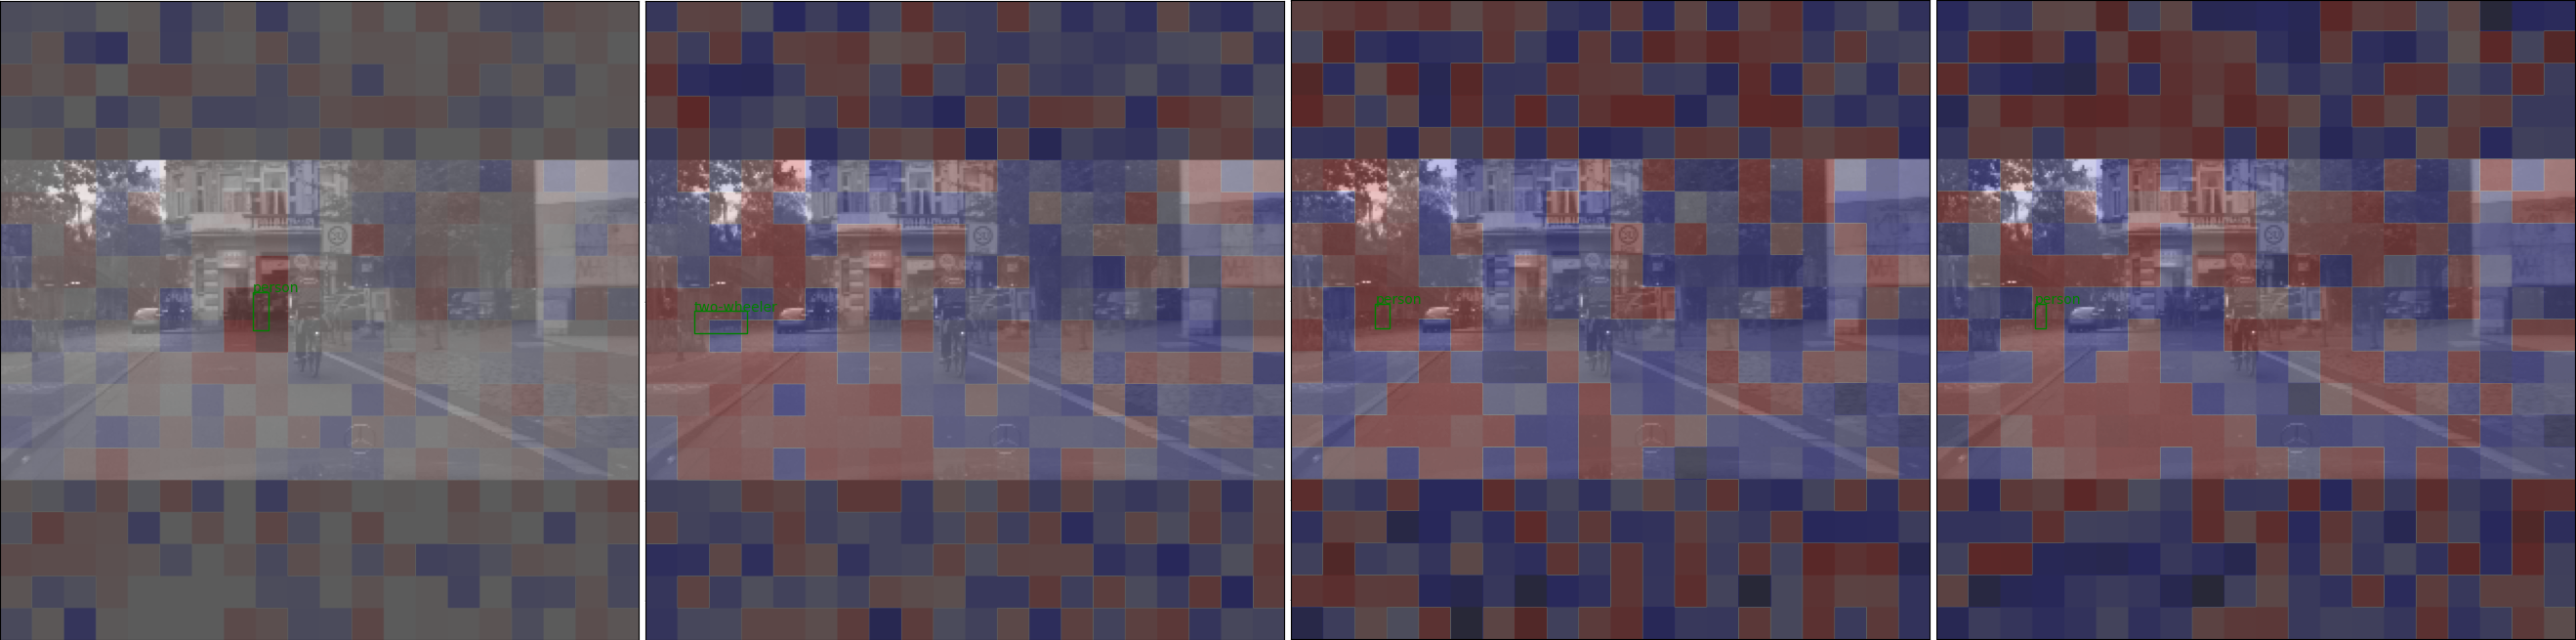
\includegraphics[width=\textwidth]{figures/output2,2}
        \caption{SHAP results}\label{fig:SHAP_results22}
    \end{subfigure}
    \caption{SHAP results for different instances}
    \label{fig:SHAP_results_combined}
\end{figure}
\paragraph{Explanation to SHAP(Figure\ref{fig:SHAP_results_combined})}


Top Row (\ref{fig:SHAP_results2}): The overlaid SHAP visualizations suggest which areas were crucial for the model in identifying these objects, which were two cars and the bike-rider .
The highlighted regions are minimal, indicating a high-confidence detection of the object, with the model focusing specifically on the relevant parts of the image.

Top Middle Row (\ref{fig:SHAP_results20}): Here, a broader range of the image is influenced by SHAP values, with more regions showing relevance to the model's predictions.
This suggests that the model is incorporating additional contextual information, such as the surroundings or the road, to reinforce its detection decisions, as well as noise made by the lacking confidence detections of these objects.
The highlighted regions expand around the objects, likely indicating the model's reliance on environmental cues in this analysis level.

Bottom middle Row (\ref{fig:SHAP_results21}): In this row, the SHAP visualization becomes even more widespread, covering a significant portion of the image. This extensive coverage suggests that the model considers a broader context in its decision-making, potentially analyzing both relevant and less relevant areas. This could mean that the model is being influenced by more peripheral or background features, reflecting a lower confidence level or a higher sensitivity to context.

Bottom Row(\ref{fig:SHAP_results22}): This pictures are almost entirely made out of noisy shap explanations, caused by often discussed lack of confidance.

\paragraph{Explanations to EigenCAM results}
\begin{figure}[h!]
    \centering


    \begin{subfigure}[b]{0.49\textwidth}
        \centering
        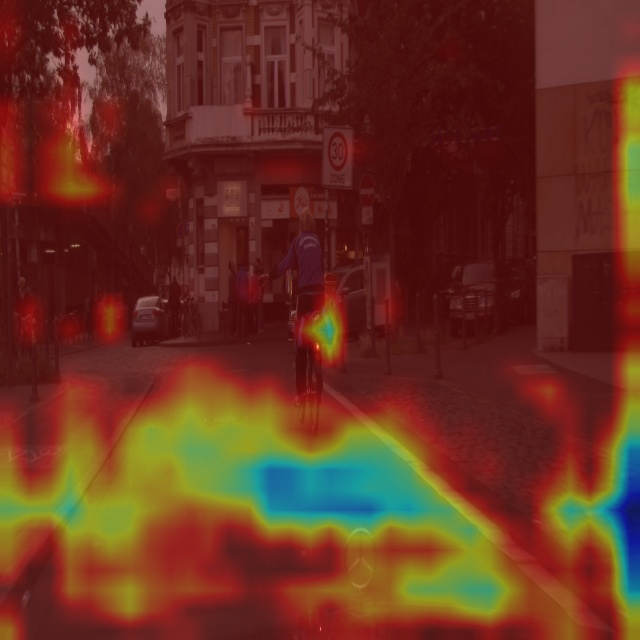
\includegraphics[width=\textwidth]{figures/bonn_000036_000019_leftImg8bit.pnglayer-2/bonn_000036_000019_leftImg8bit.png_object(0)_heatmap}
        \caption{Layer -2}
        \label{fig:b-2}
    \end{subfigure}
    \hfill
    \begin{subfigure}[b]{0.49\textwidth}
        \centering
        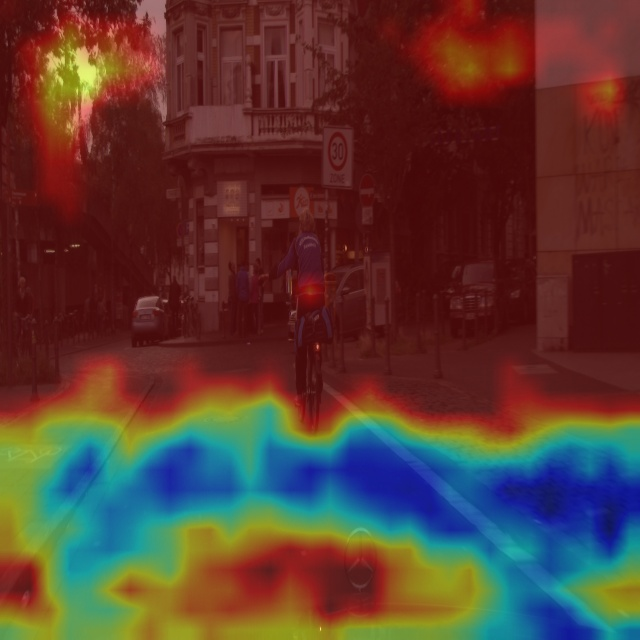
\includegraphics[width=\textwidth]{figures/bonn_000036_000019_leftImg8bit.pnglayer-3/bonn_000036_000019_leftImg8bit.png_object(0)_heatmap}
        \caption{Layer -3}
        \label{fig:b-3}
    \end{subfigure}
    \hfill
    \begin{subfigure}[b]{0.49\textwidth}
        \centering
        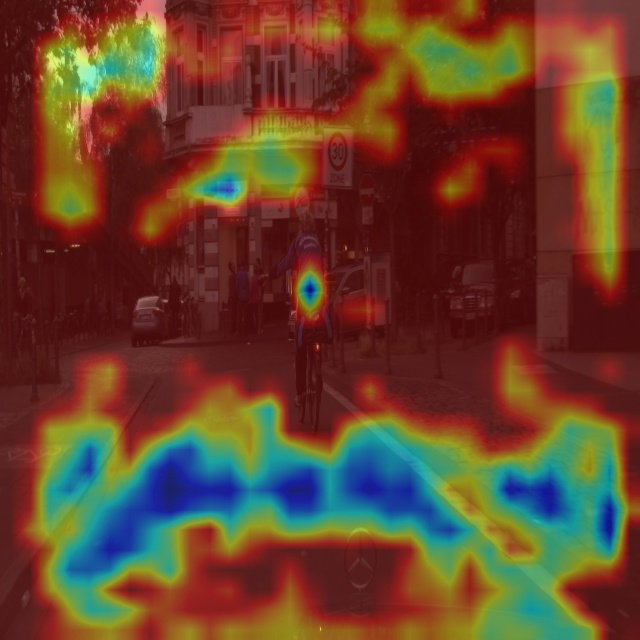
\includegraphics[width=\textwidth]{figures/bonn_000036_000019_leftImg8bit.pnglayer-4/bonn_000036_000019_leftImg8bit.png_object(0)_heatmap}
        \caption{Layer -4}
        \label{fig:b-4}
    \end{subfigure}
    \hfill
    \begin{subfigure}[b]{0.49\textwidth}
        \centering
        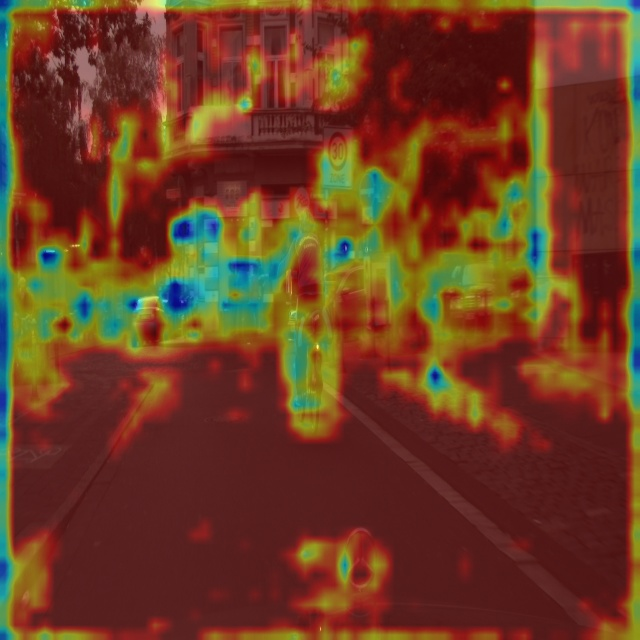
\includegraphics[width=\textwidth]{figures/bonn_000036_000019_leftImg8bit.pnglayer-5/bonn_000036_000019_leftImg8bit.png_object(0)_heatmap}
        \caption{Layer -5}
        \label{fig:b-5}
    \end{subfigure}
    \hfill

    \caption{Activation maps for the Layer -2, -3, -4, -5 for Bonn36}
    \label{fig:Bonn_000036_000019}
\end{figure}



\begin{enumerate}
    \item \textit{Layer -2 (\ref{fig:b-2})} : The activation map focuses on the central region, especially around the road and potential objects. The model detects general structures and outlines, emphasizing the primary objects in the scene.
    \item \textit{Layer -3 (\ref{fig:b-3})} : The activation expands slightly, incorporating more background elements, such as buildings and signs. The model begins to consider the broader environment around the primary objects, adding context to the detection.
    \item \textit{Layer -4 (\ref{fig:b-4})} : The activations are more dispersed across the image, covering both foreground and background elements. The model captures finer-grained features, interpreting both the main objects and additional environmental details like signs and building textures.
    \item \textit{Layer -5 (\ref{fig:b-5})} : The activation map is broad and diffuse, with high responsiveness to nearly all elements in the image, including roads, buildings, trees, and signs. The model at this stage captures complex, scene-wide patterns and high-level feature representations.
\end{enumerate}




\begin{figure}
    \centering


    \begin{subfigure}[b]{0.49\textwidth}
        \centering
        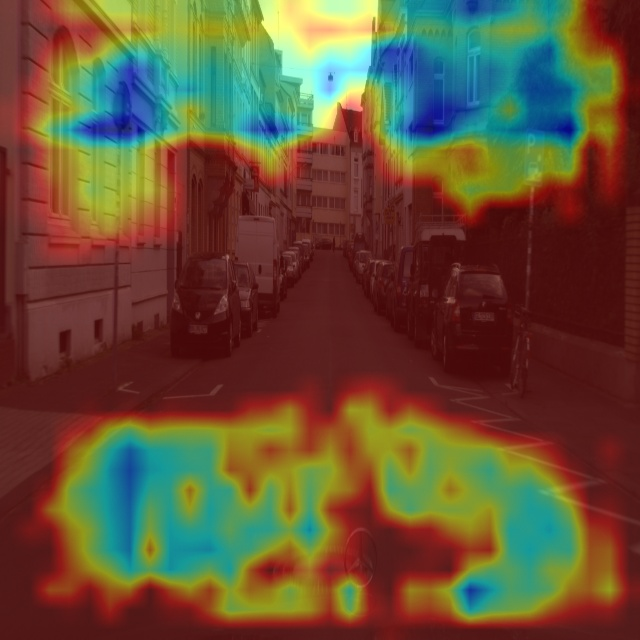
\includegraphics[width=\textwidth]{figures/bonn_000037_000019_leftImg8bit.pnglayer-2/bonn_000037_000019_leftImg8bit.png_object(0)_heatmap}
        \caption{Layer -2}
        \label{fig:c-2}
    \end{subfigure}
    \hfill
    \begin{subfigure}[b]{0.49\textwidth}
        \centering
        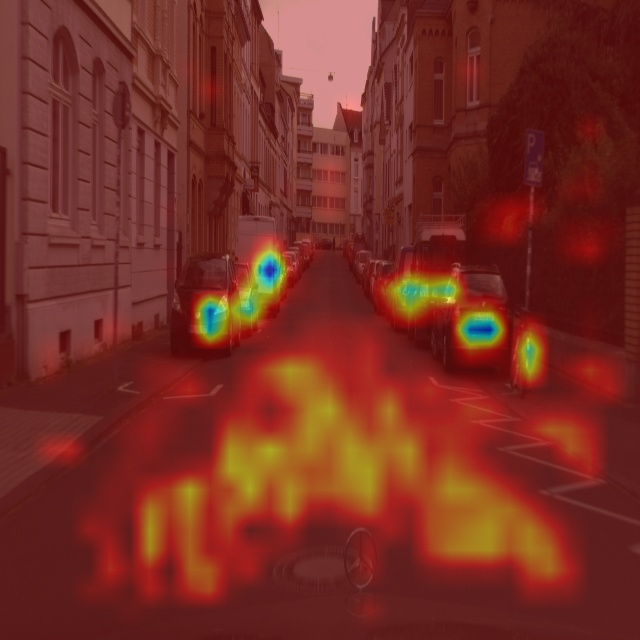
\includegraphics[width=\textwidth]{figures/bonn_000037_000019_leftImg8bit.pnglayer-3/bonn_000037_000019_leftImg8bit.png_object(0)_heatmap}
        \caption{Layer -3}
        \label{fig:c-3}
    \end{subfigure}
    \hfill
    \begin{subfigure}[b]{0.49\textwidth}
        \centering
        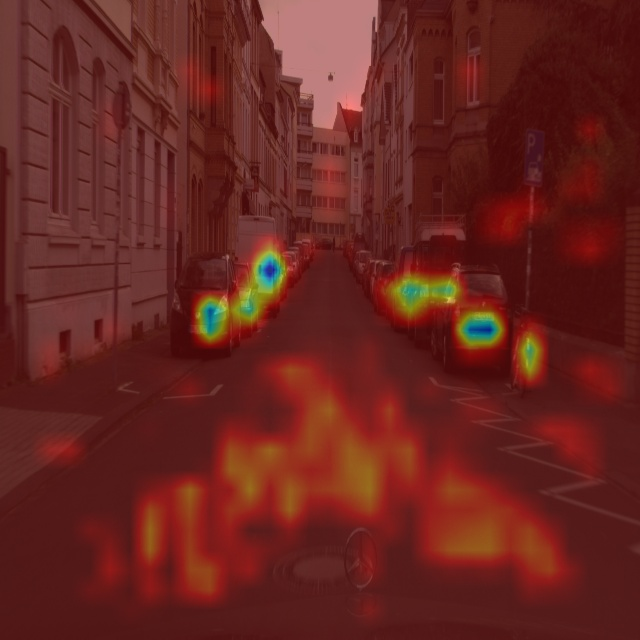
\includegraphics[width=\textwidth]{figures/bonn_000037_000019_leftImg8bit.pnglayer-4/bonn_000037_000019_leftImg8bit.png_object(0)_heatmap}
        \caption{Layer -4}
        \label{fig:c-4}
    \end{subfigure}
    \hfill
    \begin{subfigure}[b]{0.49\textwidth}
        \centering
        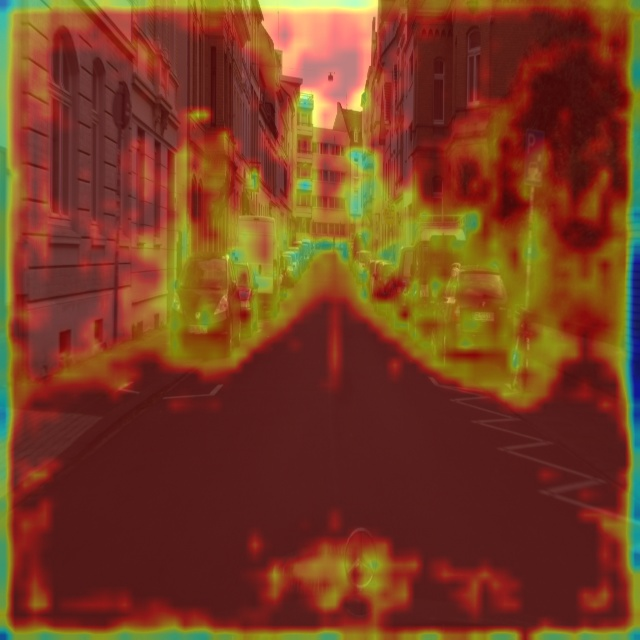
\includegraphics[width=\textwidth]{figures/bonn_000037_000019_leftImg8bit.pnglayer-5/bonn_000037_000019_leftImg8bit.png_object(0)_heatmap}
        \caption{Layer -5}
        \label{fig:c-5}
    \end{subfigure}
    \hfill
    \begin{subfigure}[b]{0.49\textwidth}
        \centering
        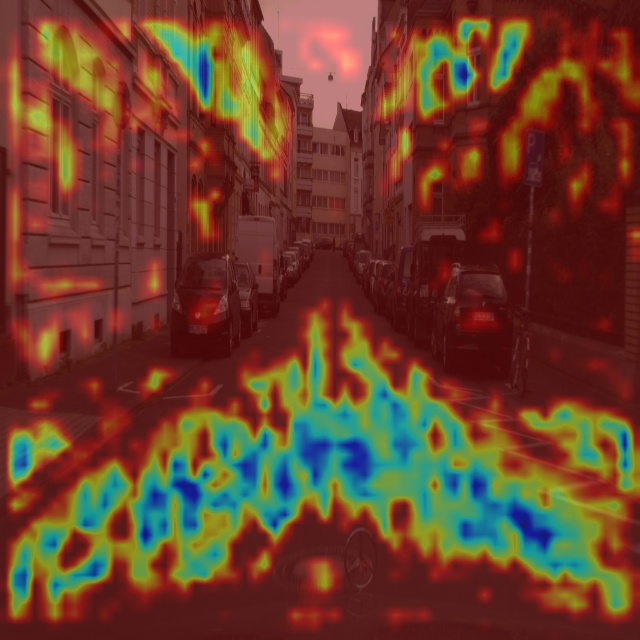
\includegraphics[width=\textwidth]{figures/bonn_000037_000019_leftImg8bit.pnglayer-6/bonn_000037_000019_leftImg8bit.png_object(0)_heatmap}
        \caption{Layer -6}
        \label{fig:c-6}
    \end{subfigure}
    \hfill

    \caption{Activation maps for the Layer -2, -3, -4, -5 for Bonn37}
    \label{fig:Bonn_000037_000019}
\end{figure}
\begin{enumerate}
    \item \textit{Layer -2 (\ref{fig:c-2})}: The activation map shows focus on both the top and bottom regions of the image, capturing general structural elements, such as the sky at the top and the street at the bottom. This layer mainly highlights broad spatial features without much fine detail.
    \item \textit{Layer -3 (\ref{fig:c-3})}: Activations become more specific, with focus on distinct points along the street. This suggests that the model is beginning to identify specific objects or areas of interest along the roadway, possibly focusing on features relevant to the street layout or potential objects in the environment.
    \item \textit{Layer -4 (\ref{fig:c-4})}: The model's focus widens, capturing both sides of the street more prominently, with activations spreading across buildings and other elements lining the road. This indicates a balance between object-specific and context-specific features, as the model integrates more scene context.
    \item \textit{Layer -5 (\ref{fig:c-5})}: The activation is more expansive, covering almost the entire image, particularly emphasizing areas surrounding the street. This layer appears to interpret larger, scene-wide patterns, possibly identifying the overall structure of the street and surrounding buildings.
    \item \textit{Layer -6 (\ref{fig:c-6})}:  Activations spread densely across the image, with a particular focus on the street's length and the buildings lining it. This deep layer captures high-level abstractions, incorporating nearly the entire scene, reflecting the model's comprehensive understanding of the spatial layout and contextual details.

\end{enumerate}

\subsection{Takeaways}\label{subsec:takeaways-and-suggestions-for-future-development}


Notable advancements have been made in the interpretation and explanation of the behaviours exhibited by computer vision models, particularly through the application of SHAP and EigenCAM.
These tools have facilitated a more profound comprehension of the decision-making processes of intricate models, thereby offering a more transparent view of the manner in which these models prioritise and process visual information in different contexts.
In particular, SHAP facilitated interpretability by decomposing model predictions into feature contributions.
EigenCAM, on the other hand, used activation-based heat maps to visualise the model's spatial awareness.

While the results of LIME  were less conclusive in this context, possibly due to challenges in its level of complexity compared to the model's architecture, the combined use of SHAP and EigenCAM successfully illustrated the potential for effective and detailed visualisations of model interpretations.
By observing SHAP and EigenCAM outputs on the same image, we were able to achieve a more comprehensive view of model processing, providing a multi-faceted perspective on how the model detects and evaluates objects.
This approach represents a step towards a comprehensive, global understanding of model behaviour through the integration of individual, local interpretations, where the strengths of each method complement the limitations of the other.

The robustness and accuracy of Yolov8 on the Cityscapes dataset further validated its ability to handle complex real-world scenes, particularly urban environments where object detection tasks can be challenging due to varying object scales, densities and positions. Yolov8 demonstrated superior performance in accurately identifying a wide range of objects within the dataset - such as pedestrians and different vehicles, - across different spatial arrangements, reflecting its resilience and adaptability to real-world applications.
This consistency across different scenarios within the Cityscapes dataset underscores Yolov8's potential for use in applications that require high precision, such as autonomous driving and urban planning.

The successful application of Yolov8 in the combination with interpretability methods such as SHAP and EigenCAM highlights a promising path for future computer vision models.
This combined approach suggests that powerful models can also be interpretable, promoting transparency without compromising performance.
This integration of interpretability tools with powerful models such as Yolov8 offers exciting possibilities for future work, such as real-time applications where both accuracy and transparency are paramount, ultimately contributing to the development of trustworthy, interpretable and powerful computer vision systems.

\subsection{Directions for further development}\label{subsec:dircetions-for-further-development}

Although this project has made considerable progress in clarifying the functioning of models in the domain of computer vision, there are still numerous avenues for further investigation and development.

Firstly, enhancing the interpretability of underperforming methods, such as LIME, could improve the consistency and reliability of model explanations across various instances.
Further investigation into parameter tuning or alternative implementations of LIME may facilitate the development of more robust explanations.

Furthermore, it would be beneficial to implement other, less well-known methods, or to revisit the approaches discussed in previous subsections (\ref{sec:model-interpretation}), such as adversarial-based interpretation methods, e.g. Anchor\cite{LIANG2021168}.
Additionally, EigenGradCAM could be utilized or another model-specific method could be employed to gain a deeper comprehension of the model's internal operations by elucidating the training process.

Furthermore, the integration of interpretability techniques, such as SHAP and EigenCAM, into real-time applications represents a promising avenue for future research.
Further work could concentrate on optimising these methods to operate effectively in conjunction with the model.

An expansion of the interpretability framework to include other datasets beyond Cityscapes would serve to further test the model's adaptability and the scalability of the interpretability methods across different environments. In addition, the incorporation of a more extensive range of data could facilitate a more comprehensive understanding of the model's generalisability and limitations.

Finally, efforts could be directed towards the development of unified visualisation tools that allow for dynamic, interactive exploration of combined interpretations from multiple methods.
Such tools would enable researchers and practitioners to better analyse, understand, and refine model behaviour across complex tasks, ultimately fostering greater trust and transparency in computer vision systems.

% Summary
%~~~~~~~~~~~~~~~~~~~~~~~~~~~~~~~~~~~~~~~~~~~~~~~~~~~~~~~~~~~~~~~~~~~~~~~~~~~~~~~~~~~~~~



% Acknowledgements
%~~~~~~~~~~~~~~~~~~~~~~~~~~~~~~~~~~~~~~~~~~~~~~~~~~~~~~~~~~~~~~~~~~~~~~~~~~~~~~~~~~~~~~
%%----------------------------------------------------------------------------
\chapter*{\koszonetnyilvanitas}\addcontentsline{toc}{chapter}{\koszonetnyilvanitas}
%----------------------------------------------------------------------------

I would like to express my deepest gratitude to my parents, Dr. Krisztián Nyilas and Ildikó Nyilasné Mészáros, for their unwavering support and encouragement throughout this journey. I am also sincerely thankful to my girlfriend, Anett Bakos, whose understanding and help with  helped me stay focused.

Special thanks to my consultant, Dr. Gábor Hullám, for his invaluable guidance and insights, which greatly enriched this work.

I am profoundly grateful to all who have supported me along the way.


% List of Figures, Tables
%~~~~~~~~~~~~~~~~~~~~~~~~~~~~~~~~~~~~~~~~~~~~~~~~~~~~~~~~~~~~~~~~~~~~~~~~~~~~~~~~~~~~~~
\listoffigures\addcontentsline{toc}{chapter}{\listfigurename}
%\listoftables\addcontentsline{toc}{chapter}{\listtablename}


% Bibliography
%~~~~~~~~~~~~~~~~~~~~~~~~~~~~~~~~~~~~~~~~~~~~~~~~~~~~~~~~~~~~~~~~~~~~~~~~~~~~~~~~~~~~~~
\addcontentsline{toc}{chapter}{\bibname}
\bibliography{bib/mybib}


% Appendix
%~~~~~~~~~~~~~~~~~~~~~~~~~~~~~~~~~~~~~~~~~~~~~~~~~~~~~~~~~~~~~~~~~~~~~~~~~~~~~~~~~~~~~~
%include{content/appendices}

%\label{page:last}
\end{spacing}
\end{document}
